% Options for packages loaded elsewhere
\PassOptionsToPackage{unicode}{hyperref}
\PassOptionsToPackage{hyphens}{url}
\PassOptionsToPackage{dvipsnames,svgnames*,x11names*}{xcolor}
%
\documentclass[
]{book}
\usepackage{lmodern}
\usepackage{amssymb,amsmath}
\usepackage{ifxetex,ifluatex}
\ifnum 0\ifxetex 1\fi\ifluatex 1\fi=0 % if pdftex
  \usepackage[T1]{fontenc}
  \usepackage[utf8]{inputenc}
  \usepackage{textcomp} % provide euro and other symbols
\else % if luatex or xetex
  \usepackage{unicode-math}
  \defaultfontfeatures{Scale=MatchLowercase}
  \defaultfontfeatures[\rmfamily]{Ligatures=TeX,Scale=1}
\fi
% Use upquote if available, for straight quotes in verbatim environments
\IfFileExists{upquote.sty}{\usepackage{upquote}}{}
\IfFileExists{microtype.sty}{% use microtype if available
  \usepackage[]{microtype}
  \UseMicrotypeSet[protrusion]{basicmath} % disable protrusion for tt fonts
}{}
\makeatletter
\@ifundefined{KOMAClassName}{% if non-KOMA class
  \IfFileExists{parskip.sty}{%
    \usepackage{parskip}
  }{% else
    \setlength{\parindent}{0pt}
    \setlength{\parskip}{6pt plus 2pt minus 1pt}}
}{% if KOMA class
  \KOMAoptions{parskip=half}}
\makeatother
\usepackage{xcolor}
\IfFileExists{xurl.sty}{\usepackage{xurl}}{} % add URL line breaks if available
\IfFileExists{bookmark.sty}{\usepackage{bookmark}}{\usepackage{hyperref}}
\hypersetup{
  pdftitle={Matlab Toolbox Heterogeneous Agents Dynamic Programming},
  pdfauthor={Fan Wang},
  colorlinks=true,
  linkcolor=Maroon,
  filecolor=Maroon,
  citecolor=Blue,
  urlcolor=blue,
  pdfcreator={LaTeX via pandoc}}
\urlstyle{same} % disable monospaced font for URLs
\usepackage{longtable,booktabs}
% Correct order of tables after \paragraph or \subparagraph
\usepackage{etoolbox}
\makeatletter
\patchcmd\longtable{\par}{\if@noskipsec\mbox{}\fi\par}{}{}
\makeatother
% Allow footnotes in longtable head/foot
\IfFileExists{footnotehyper.sty}{\usepackage{footnotehyper}}{\usepackage{footnote}}
\makesavenoteenv{longtable}
\usepackage{graphicx,grffile}
\makeatletter
\def\maxwidth{\ifdim\Gin@nat@width>\linewidth\linewidth\else\Gin@nat@width\fi}
\def\maxheight{\ifdim\Gin@nat@height>\textheight\textheight\else\Gin@nat@height\fi}
\makeatother
% Scale images if necessary, so that they will not overflow the page
% margins by default, and it is still possible to overwrite the defaults
% using explicit options in \includegraphics[width, height, ...]{}
\setkeys{Gin}{width=\maxwidth,height=\maxheight,keepaspectratio}
% Set default figure placement to htbp
\makeatletter
\def\fps@figure{htbp}
\makeatother
\setlength{\emergencystretch}{3em} % prevent overfull lines
\providecommand{\tightlist}{%
  \setlength{\itemsep}{0pt}\setlength{\parskip}{0pt}}
\setcounter{secnumdepth}{5}
\usepackage{bbm}
\usepackage{booktabs}
\usepackage{longtable}
\usepackage{array}
\usepackage{multirow}
\usepackage{wrapfig}
\usepackage{float}
% \floatplacement{figure}{H}
\usepackage[labelformat = empty]{caption}
\usepackage{colortbl}
\usepackage{pdflscape}
\usepackage{tabu}
\usepackage{threeparttable}
\usepackage{threeparttablex}
\usepackage[normalem]{ulem}
\usepackage{makecell}
\usepackage{xcolor}
\usepackage{geometry}
\geometry{
	a4paper,
	left=1.0in,
	right=1.0in,
	top=1.0in,
	bottom=1.0in,
}
\setcounter{secnumdepth}{5}
\setcounter{tocdepth}{5}
\usepackage[]{natbib}
\bibliographystyle{apalike}

\title{Matlab Toolbox Heterogeneous Agents Dynamic Programming}
\author{Fan Wang}
\date{2020-06-28}

\begin{document}
\maketitle

{
\hypersetup{linkcolor=}
\setcounter{tocdepth}{1}
\tableofcontents
}
\hypertarget{preface}{%
\chapter*{Preface}\label{preface}}
\addcontentsline{toc}{chapter}{Preface}

This is a work-in-progress Matlab package consisting of functions that facilitate Dynamic Programming and Related Tasks. Materials gathered from various \href{https://fanwangecon.github.io/research}{projects} in which Matlab code is used. Files are the \href{https://github.com/FanWangEcon/MEconTools}{MEconTools} repository. Matlab files are linked below by section with livescript files. Tested with \href{https://www.mathworks.com/products/matlab.html}{Matlab} 2019a \citep{matlab}.

This bookdown file is a collection of mlx based vignettes for functions that are available from \href{https://github.com/FanWangEcon/MEconTools}{MEconTools}. Each Vignette file contains various examples for invoking each function. The goal of this repository is to make it easier to find/re-use codes produced for various projects.

From other repositories: For dynamic borrowing and savings problems, see \href{https://fanwangecon.github.io/CodeDynaAsset/}{Dynamic Asset Repository}; For code examples, see also \href{https://fanwangecon.github.io/R4Econ/}{R Example Code}, \href{https://fanwangecon.github.io/M4Econ/}{Matlab Example Code}, and \href{https://fanwangecon.github.io/Stata4Econ/}{Stata Example Code}; For intro stat with R, see \href{https://fanwangecon.github.io/Stat4Econ/}{Intro Statistics for Undergraduates}, and intro Math with Matlab, see \href{https://fanwangecon.github.io/Math4Econ/}{Intro Mathematics for Economists}. See \href{https://github.com/FanWangEcon}{here} for all of \href{https://fanwangecon.github.io/}{Fan}'s public repositories.

The site is built using \href{https://bookdown.org/}{Bookdown} \citep{R-bookdown}.

Please contact \href{https://fanwangecon.github.io/}{FanWangEcon} for issues or problems.

\hypertarget{summarize-policy-and-value}{%
\chapter{Summarize Policy and Value}\label{summarize-policy-and-value}}

\hypertarget{ff_summ_nd_array-examples}{%
\section{FF\_SUMM\_ND\_ARRAY Examples}\label{ff_summ_nd_array-examples}}

\begin{quote}
Go back to \href{http://fanwangecon.github.io/}{fan}'s \href{https://fanwangecon.github.io/MEconTools/}{MEconTools} Toolbox (\href{https://fanwangecon.github.io/MEconTools/bookdown}{bookdown}), \href{https://fanwangecon.github.io/M4Econ/}{Matlab Code Examples} Repository (\href{https://fanwangecon.github.io/M4Econ/bookdown}{bookdown}), or \href{https://fanwangecon.github.io/Math4Econ/}{Math for Econ with Matlab} Repository (\href{https://fanwangecon.github.io/Math4Econ/bookdown}{bookdown}).
\end{quote}

This is the example vignette for function:
\href{https://github.com/FanWangEcon/MEconTools/blob/master/MEconTools/summ/ff_summ_nd_array.m}{\textbf{ff\_summ\_nd\_array}}
from the \href{https://fanwangecon.github.io/MEconTools/}{\textbf{MEconTools
Package}}\textbf{.} This function
summarizes policy and value functions over states.

\hypertarget{test-ff_summ_nd_array-defaults}{%
\subsection{Test FF\_SUMM\_ND\_ARRAY Defaults}\label{test-ff_summ_nd_array-defaults}}

Call the function with defaults.

\begin{verbatim}
ff_summ_nd_array();

xxx  Summ over (a,z), condi age as cols, kids/marriage as rows  xxxxxxxxxxxxxxxxxxxxxxxxxxx
    group    marry    kids    mean_age_18    mean_age_19    mean_age_20    mean_age_21
    _____    _____    ____    ___________    ___________    ___________    ___________

      1        0       1        0.52456        0.51689        0.48412        0.54526  
      2        1       1        0.49355        0.52906         0.5583        0.47342  
      3        0       2        0.49085        0.51315        0.45158        0.43201  
      4        1       2        0.58096        0.50596        0.47985        0.58791  
      5        0       3        0.57811         0.6068        0.55221        0.50677  
      6        1       3        0.53023        0.49258        0.48728        0.43352  
      7        0       4        0.50339        0.48449        0.53618        0.45993  
      8        1       4        0.44418         0.5223        0.55657        0.48583  
\end{verbatim}

\hypertarget{test-ff_summ_nd_array-with-random-2-dimensional-matrix}{%
\subsection{Test FF\_SUMM\_ND\_ARRAY with Random 2 Dimensional Matrix}\label{test-ff_summ_nd_array-with-random-2-dimensional-matrix}}

Summarize over 6 dimensional array, iteratively change how many
dimensions to group over.

First, generate matrix:

\begin{verbatim}
st_title = "Random 2D dimensional Array Testing Summarizing";
rng(123)
mn_polval = rand(5,4);
bl_print_table = true;
ar_st_stats = ["mean"];
cl_mp_datasetdesc = {};
cl_mp_datasetdesc{1} = containers.Map({'name', 'labval'}, ...
    {'a', linspace(0,1,size(mn_polval,1))});
cl_mp_datasetdesc{2} = containers.Map({'name', 'labval'}, ...
    {'z', linspace(-1,1,size(mn_polval,2))});
disp(mn_polval);

    0.6965    0.4231    0.3432    0.7380
    0.2861    0.9808    0.7290    0.1825
    0.2269    0.6848    0.4386    0.1755
    0.5513    0.4809    0.0597    0.5316
    0.7195    0.3921    0.3980    0.5318
\end{verbatim}

Second, show the entire matrix (no labels):

\begin{verbatim}
it_aggd = 0; 
bl_row = 1; 
ff_summ_nd_array(st_title, mn_polval, bl_print_table, ar_st_stats, it_aggd, bl_row);

xxx  Random 2D dimensional Array Testing Summarizing  xxxxxxxxxxxxxxxxxxxxxxxxxxx
    group    vardim2    mean_vardim1_1    mean_vardim1_2    mean_vardim1_3    mean_vardim1_4    mean_vardim1_5
    _____    _______    ______________    ______________    ______________    ______________    ______________

      1         1          0.69647           0.28614           0.22685            0.55131          0.71947    
      2         2          0.42311           0.98076           0.68483            0.48093          0.39212    
      3         3          0.34318           0.72905           0.43857           0.059678          0.39804    
      4         4            0.738           0.18249           0.17545            0.53155          0.53183    
\end{verbatim}

Third, rotate row and column, and now with labels:

\begin{verbatim}
it_aggd = 0; 
bl_row = 1; 
ar_permute = [2,1];
ff_summ_nd_array(st_title, mn_polval, bl_print_table, ar_st_stats, it_aggd, bl_row, ...
    cl_mp_datasetdesc, ar_permute);

xxx  Random 2D dimensional Array Testing Summarizing  xxxxxxxxxxxxxxxxxxxxxxxxxxx
    group     a      mean_z__1    mean_z__0_33333    mean_z_0_33333    mean_z_1
    _____    ____    _________    _______________    ______________    ________

      1         0     0.69647         0.42311            0.34318         0.738 
      2      0.25     0.28614         0.98076            0.72905       0.18249 
      3       0.5     0.22685         0.68483            0.43857       0.17545 
      4      0.75     0.55131         0.48093           0.059678       0.53155 
      5         1     0.71947         0.39212            0.39804       0.53183 
\end{verbatim}

Fourth, dimension one as columns, average over dim 2:

\begin{verbatim}
it_aggd = 1; 
bl_row = 1; 
ff_summ_nd_array(st_title, mn_polval, bl_print_table, ar_st_stats, it_aggd, bl_row, ...
    cl_mp_datasetdesc);

xxx  Random 2D dimensional Array Testing Summarizing  xxxxxxxxxxxxxxxxxxxxxxxxxxx
    group    x    mean_z__1    mean_z__0_33333    mean_z_0_33333    mean_z_1
    _____    _    _________    _______________    ______________    ________

      1      1     0.49605         0.59235            0.3937        0.43186 
\end{verbatim}

Fifth, dimension one as rows, average over dim 2:

\begin{verbatim}
it_aggd = 1; 
bl_row = 0; 
ff_summ_nd_array(st_title, mn_polval, bl_print_table, ar_st_stats, it_aggd, bl_row, ...
    cl_mp_datasetdesc);

xxx  Random 2D dimensional Array Testing Summarizing  xxxxxxxxxxxxxxxxxxxxxxxxxxx
    group       z         sum       mean        std      coefvari      min         max  
    _____    ________    ______    _______    _______    ________    ________    _______

      1            -1    2.4802    0.49605    0.22895     2.1666      0.22685    0.71947
      2      -0.33333    2.9617    0.59235    0.24524     2.4154      0.39212    0.98076
      3       0.33333    1.9685     0.3937    0.23907     1.6468     0.059678    0.72905
      4             1    2.1593    0.43186    0.24575     1.7573      0.17545      0.738
\end{verbatim}

Sixth, dimension two as rows, average over dim 1:

\begin{verbatim}
ar_permute = [2,1];
it_aggd = 1; 
bl_row = 0; 
ff_summ_nd_array(st_title, mn_polval, bl_print_table, ar_st_stats, it_aggd, bl_row, ...
    cl_mp_datasetdesc, ar_permute);

xxx  Random 2D dimensional Array Testing Summarizing  xxxxxxxxxxxxxxxxxxxxxxxxxxx
    group     a       sum       mean        std      coefvari      min         max  
    _____    ____    ______    _______    _______    ________    ________    _______

      1         0    2.2007    0.55019    0.19636     2.8019      0.34318      0.738
      2      0.25    2.1784    0.54461    0.37514     1.4518      0.18249    0.98076
      3       0.5    1.5257    0.38143    0.23212     1.6432      0.17545    0.68483
      4      0.75    1.6235    0.40587    0.23269     1.7443     0.059678    0.55131
      5         1    2.0415    0.51036    0.15361     3.3226      0.39212    0.71947
\end{verbatim}

\hypertarget{test-ff_summ_nd_array-with-random-6-dimensional-matrix}{%
\subsection{Test FF\_SUMM\_ND\_ARRAY with Random 6 Dimensional Matrix}\label{test-ff_summ_nd_array-with-random-6-dimensional-matrix}}

Summarize over 6 dimensional array, iteratively change how many
dimensions to group over.

First, generate matrix:

\begin{verbatim}
st_title = "Random ND dimensional Array Testing Summarizing";
rng(123)
mn_polval = rand(8,7,6,5,4,3);
bl_print_table = true;
ar_st_stats = ["mean"];
\end{verbatim}

Second, summarize over the first four dimensions, row group others:

\begin{verbatim}
it_aggd = 4; 
bl_row = 0; 
ff_summ_nd_array(st_title, mn_polval, bl_print_table, ar_st_stats, it_aggd, bl_row);

xxx  Random ND dimensional Array Testing Summarizing  xxxxxxxxxxxxxxxxxxxxxxxxxxx
    group    vardim5    vardim6     sum       mean        std      coefvari       min          max  
    _____    _______    _______    ______    _______    _______    ________    __________    _______

      1         1          1       836.78    0.49808    0.29255     1.7026     8.1888e-05    0.99964
      2         2          1       842.15    0.50128    0.28968     1.7305     6.7838e-05    0.99936
      3         3          1       831.45    0.49491    0.28851     1.7154     0.00091373    0.99989
      4         4          1        843.9    0.50232    0.28154     1.7842     0.00012471    0.99731
      5         1          2       838.99     0.4994     0.2911     1.7156     0.00029749    0.99938
      6         2          2       830.81    0.49453    0.28634     1.7271     0.00027113     0.9992
      7         3          2       832.59    0.49559    0.28682     1.7279     0.00035994    0.99936
      8         4          2       820.42    0.48835    0.29032     1.6821     0.00096259    0.99896
      9         1          3       870.56    0.51819    0.29111     1.7801      0.0010616    0.99951
     10         2          3       854.68    0.50874    0.28458     1.7877       0.001884    0.99965
     11         3          3       838.29    0.49898     0.2891      1.726      0.0019192    0.99945
     12         4          3       842.83    0.50169     0.2877     1.7438     0.00016871    0.99963
\end{verbatim}

Third, summarize over the first four dimensions, column group 5th, and
row group others:

\begin{verbatim}
it_aggd = 4; 
bl_row = 1; 
ff_summ_nd_array(st_title, mn_polval, bl_print_table, ["sum"], it_aggd, bl_row);

xxx  Random ND dimensional Array Testing Summarizing  xxxxxxxxxxxxxxxxxxxxxxxxxxx
    group    vardim6    sum_vardim5_1    sum_vardim5_2    sum_vardim5_3    sum_vardim5_4
    _____    _______    _____________    _____________    _____________    _____________

      1         1          836.78           842.15           831.45            843.9    
      2         2          838.99           830.81           832.59           820.42    
      3         3          870.56           854.68           838.29           842.83    
\end{verbatim}

Fourth, summarize over the first five dimensions, column group 6th, no
row groups:

\begin{verbatim}
it_aggd = 5;
bl_row = 1; 
ff_summ_nd_array(st_title, mn_polval, bl_print_table, ["mean", "std"], it_aggd, bl_row);

xxx  Random ND dimensional Array Testing Summarizing  xxxxxxxxxxxxxxxxxxxxxxxxxxx
    group    x    mean_vardim6_1    mean_vardim6_2    mean_vardim6_3    std_vardim6_1    std_vardim6_2    std_vardim6_3
    _____    _    ______________    ______________    ______________    _____________    _____________    _____________

      1      1       0.49915           0.49447            0.5069           0.28805          0.28862          0.28816   
\end{verbatim}

Fifth, summarize over all six dimensions, summary statistics over the
entire dataframe:

\begin{verbatim}
it_aggd = 6;
bl_row = 0; 
ff_summ_nd_array(st_title, mn_polval, bl_print_table, ar_st_stats, it_aggd, bl_row);

xxx  Random ND dimensional Array Testing Summarizing  xxxxxxxxxxxxxxxxxxxxxxxxxxx
    group    x     sum      mean        std      coefvari       min          max  
    _____    _    _____    _______    _______    ________    __________    _______

      1      1    10083    0.50017    0.28831     1.7349     6.7838e-05    0.99989
\end{verbatim}

\hypertarget{test-ff_summ_nd_array-with-random-7-dimensional-matrix-with-all-parameters}{%
\subsection{Test FF\_SUMM\_ND\_ARRAY with Random 7 Dimensional Matrix with All Parameters}\label{test-ff_summ_nd_array-with-random-7-dimensional-matrix-with-all-parameters}}

Given a random seven dimensional matrix, average over the 2nd, 4th and
5th dimensionals. Show as row groups the 3, 6 and 7th dimensions, and
row groups the 1st dimension. Show Coefficient of Variation only.

\begin{verbatim}
st_title = "avg VALUE 2+4+5th dims. groups 3+6+7th dims, and row groups the 1st dim.";
rng(123)
mn_polval = rand(3,10,2,10,10,2,3);
ar_permute = [2,4,5,1,3,6,7];
bl_print_table = true;
ar_st_stats = ["coefvari"];
it_aggd = 3; % mean over 3 dims
bl_row = 1; % one var for row group
cl_mp_datasetdesc = {};
cl_mp_datasetdesc{1} = containers.Map({'name', 'labval'}, ...
    {'age', [18, 19, 20]});
cl_mp_datasetdesc{2} = containers.Map({'name', 'labval'}, ...
    {'savings', linspace(0,1,10)});
cl_mp_datasetdesc{3} = containers.Map({'name', 'labval'}, ...
    {'borrsave', [-1,+1]});
cl_mp_datasetdesc{4} = containers.Map({'name', 'labval'}, ...
    {'shocka', linspace(-5,5,10)});
cl_mp_datasetdesc{5} = containers.Map({'name', 'labval'}, ...
    {'shockb', linspace(-5,5,10)});
cl_mp_datasetdesc{6} = containers.Map({'name', 'labval'}, ...
    {'marry', [0,1]});
cl_mp_datasetdesc{7} = containers.Map({'name', 'labval'}, ...
    {'region', [1,2,3]});
% call function
ff_summ_nd_array(st_title, mn_polval, bl_print_table, ar_st_stats, it_aggd, bl_row, cl_mp_datasetdesc, ar_permute);

xxx  avg VALUE 2+4+5th dims. groups 3+6+7th dims, and row groups the 1st dim.  xxxxxxxxxxxxxxxxxxxxxxxxxxx
    group    borrsave    marry    region    cv_age_18    cv_age_19    cv_age_20
    _____    ________    _____    ______    _________    _________    _________

      1         -1         0        1        1.7607       1.7534       1.7065  
      2          1         0        1        1.6566       1.7501       1.7042  
      3         -1         1        1        1.6608       1.7658       1.7291  
      4          1         1        1         1.756       1.7479       1.7606  
      5         -1         0        2        1.7314       1.7506        1.786  
      6          1         0        2        1.7347        1.728        1.738  
      7         -1         1        2        1.7811        1.755       1.7568  
      8          1         1        2        1.7445       1.7398       1.7746  
      9         -1         0        3        1.7025       1.7286         1.69  
     10          1         0        3          1.74       1.7549       1.7356  
     11         -1         1        3        1.7147       1.7287       1.7341  
     12          1         1        3        1.7919       1.7313       1.7452  
\end{verbatim}

\vspace{1em}

\hypertarget{distributional-analysis}{%
\chapter{Distributional Analysis}\label{distributional-analysis}}

\hypertarget{ff_simu_stats-examples}{%
\section{FF\_SIMU\_STATS Examples}\label{ff_simu_stats-examples}}

\begin{quote}
Go back to \href{http://fanwangecon.github.io/}{fan}'s \href{https://fanwangecon.github.io/MEconTools/}{MEconTools} Toolbox (\href{https://fanwangecon.github.io/MEconTools/bookdown}{bookdown}), \href{https://fanwangecon.github.io/M4Econ/}{Matlab Code Examples} Repository (\href{https://fanwangecon.github.io/M4Econ/bookdown}{bookdown}), or \href{https://fanwangecon.github.io/Math4Econ/}{Math for Econ with Matlab} Repository (\href{https://fanwangecon.github.io/Math4Econ/bookdown}{bookdown}).
\end{quote}

This is the example vignette for function:
\href{https://github.com/FanWangEcon/MEconTools/blob/master/MEconTools/stats/ff_simu_stats.m}{\textbf{ff\_simu\_stats}}
from the \href{https://fanwangecon.github.io/MEconTools/}{\textbf{MEconTools
Package}}\textbf{.} This is a
gate-way function that computes mean, percentiles, covariance etc
between several variables.

\hypertarget{test-ff_simu_stats-defaults}{%
\subsection{Test FF\_SIMU\_STATS Defaults}\label{test-ff_simu_stats-defaults}}

Call the function with defaults.

\begin{verbatim}
ff_simu_stats();

xxx tb_outcomes: all stats xxx
    OriginalVariableNames     cl_mt_pol_a    cl_mt_pol_c
    ______________________    ___________    ___________

    {'mean'              }     -0.11081          8.8423 
    {'sd'                }       4.1239          6.5845 
    {'coefofvar'         }      -37.215         0.74466 
    {'min'               }           -7         -6.3772 
    {'max'               }            9          21.786 
    {'pYis0'             }     0.064259               0 
    {'pYls0'             }      0.54867        0.027329 
    {'pYgr0'             }      0.38707         0.97267 
    {'pYisMINY'          }     0.051764        0.015232 
    {'pYisMAXY'          }     0.027329        0.046484 
    {'p1'                }           -7         -6.3772 
    {'p10'               }           -6         0.27238 
    {'p25'               }           -3          5.2138 
    {'p50'               }           -1          6.5321 
    {'p75'               }            3          13.799 
    {'p90'               }            5          16.887 
    {'p99'               }            9          21.786 
    {'fl_cov_cl_mt_pol_a'}       17.007         -22.084 
    {'fl_cor_cl_mt_pol_a'}            1        -0.81327 
    {'fl_cov_cl_mt_pol_c'}      -22.084          43.356 
    {'fl_cor_cl_mt_pol_c'}     -0.81327               1 
    {'fracByP1'          }       3.2699       -0.010985 
    {'fracByP10'         }       5.9889       -0.013362 
    {'fracByP25'         }       14.165        0.041007 
    {'fracByP50'         }       16.208          0.1893 
    {'fracByP75'         }       12.702         0.59539 
    {'fracByP90'         }       6.6611          0.8307 
    {'fracByP99'         }            1               1 
\end{verbatim}

\hypertarget{test-ff_simu_stats-four-states-points-matrix}{%
\subsection{Test FF\_SIMU\_STATS Four States-Points Matrix}\label{test-ff_simu_stats-four-states-points-matrix}}

Over some (a,z) states that is 3 by 3, c matrix, generate all stats

\begin{verbatim}
% Set Parameters
mt_x_of_s = [1, 2,  3.0;...
             3, 1,  1.5;...
             4, 3,  2.0];
mt_y_of_s = [2, -10, 9.0;...
             5, 1.1,3.0;...
             1, 3,  -1.5];
mt_z_of_s = [1.1, 2,3.3;...
             2.3, 1,1.5;...
             4, 2.5,2.0];
mp_cl_mt_xyz_of_s = containers.Map('KeyType','char', 'ValueType','any');
mp_cl_mt_xyz_of_s('cl_mt_x_of_s') = {mt_x_of_s, zeros(1)};
mp_cl_mt_xyz_of_s('cl_mt_y_of_s') = {mt_y_of_s, zeros(1)};
mp_cl_mt_xyz_of_s('cl_mt_z_of_s') = {mt_z_of_s, zeros(1)};
mp_cl_mt_xyz_of_s('ar_st_y_name') = ["cl_mt_x_of_s", "cl_mt_y_of_s", "cl_mt_z_of_s"];
% Mass
rng(123);
mt_f_of_s = rand(size(mt_x_of_s));
mt_f_of_s = mt_f_of_s/sum(mt_f_of_s, 'all');
% Call Function
mp_cl_mt_xyz_of_s_out = ff_simu_stats(mt_f_of_s, mp_cl_mt_xyz_of_s);

xxx tb_outcomes: all stats xxx
     OriginalVariableNames     cl_mt_x_of_s    cl_mt_y_of_s    cl_mt_z_of_s
    _______________________    ____________    ____________    ____________

    {'mean'               }        2.0763          1.9323          2.0668  
    {'sd'                 }        0.9071          5.2239          0.9042  
    {'coefofvar'          }       0.43688          2.7034         0.43749  
    {'min'                }             1             -10               1  
    {'max'                }             4               9               4  
    {'pYis0'              }             0               0               0  
    {'pYls0'              }             0         0.20441               0  
    {'pYgr0'              }             1         0.79559               1  
    {'pYisMINY'           }       0.28039         0.10917         0.14247  
    {'pYisMAXY'           }      0.044922         0.19422        0.044922  
    {'p1'                 }             1             -10               1  
    {'p10'                }             1             -10               1  
    {'p25'                }             1             1.1             1.1  
    {'p50'                }             2               2               2  
    {'p75'                }             3               5             2.5  
    {'p90'                }             3               9             3.3  
    {'p99'                }             4               9               4  
    {'fl_cov_cl_mt_x_of_s'}       0.82282           1.589         0.78646  
    {'fl_cor_cl_mt_x_of_s'}             1         0.33534         0.95887  
    {'fl_cov_cl_mt_y_of_s'}         1.589          27.289          1.8353  
    {'fl_cor_cl_mt_y_of_s'}       0.33534               1         0.38856  
    {'fl_cov_cl_mt_z_of_s'}       0.78646          1.8353         0.81758  
    {'fl_cor_cl_mt_z_of_s'}       0.95887         0.38856               1  
    {'fracByP1'           }       0.13504        -0.56498        0.068934  
    {'fracByP10'          }       0.13504        -0.56498        0.068934  
    {'fracByP25'          }       0.13504        -0.53456         0.14234  
    {'fracByP50'          }       0.42991        -0.39181         0.43856  
    {'fracByP75'          }       0.91346        0.095425         0.60296  
    {'fracByP90'          }       0.91346               1         0.91306  
    {'fracByP99'          }             1               1               1  
\end{verbatim}

\hypertarget{test-ff_simu_stats-four-states-points-matrix-single-column-inputs}{%
\subsection{Test FF\_SIMU\_STATS Four States-Points Matrix Single Column Inputs}\label{test-ff_simu_stats-four-states-points-matrix-single-column-inputs}}

Same as before, but now inputs are single column, should have identical
results:

\begin{verbatim}
% Array Inputs
mp_cl_ar_xyz_of_s = containers.Map('KeyType','char', 'ValueType','any');
mp_cl_mt_xyz_of_s('cl_mt_x_of_s') = {mt_x_of_s(:), zeros(1)};
mp_cl_mt_xyz_of_s('cl_mt_y_of_s') = {mt_y_of_s(:), zeros(1)};
mp_cl_mt_xyz_of_s('cl_mt_z_of_s') = {mt_z_of_s(:), zeros(1)};
mp_cl_mt_xyz_of_s('ar_st_y_name') = ["cl_mt_x_of_s", "cl_mt_y_of_s", "cl_mt_z_of_s"];
% Call Function
mp_cl_mt_xyz_of_s_out = ff_simu_stats(mt_f_of_s(:), mp_cl_mt_xyz_of_s);

xxx tb_outcomes: all stats xxx
     OriginalVariableNames     cl_mt_x_of_s    cl_mt_y_of_s    cl_mt_z_of_s
    _______________________    ____________    ____________    ____________

    {'mean'               }        2.0763          1.9323          2.0668  
    {'sd'                 }        0.9071          5.2239          0.9042  
    {'coefofvar'          }       0.43688          2.7034         0.43749  
    {'min'                }             1             -10               1  
    {'max'                }             4               9               4  
    {'pYis0'              }             0               0               0  
    {'pYls0'              }             0         0.20441               0  
    {'pYgr0'              }             1         0.79559               1  
    {'pYisMINY'           }       0.28039         0.10917         0.14247  
    {'pYisMAXY'           }      0.044922         0.19422        0.044922  
    {'p1'                 }             1             -10               1  
    {'p10'                }             1             -10               1  
    {'p25'                }             1             1.1             1.1  
    {'p50'                }             2               2               2  
    {'p75'                }             3               5             2.5  
    {'p90'                }             3               9             3.3  
    {'p99'                }             4               9               4  
    {'fl_cov_cl_mt_x_of_s'}       0.82282           1.589         0.78646  
    {'fl_cor_cl_mt_x_of_s'}             1         0.33534         0.95887  
    {'fl_cov_cl_mt_y_of_s'}         1.589          27.289          1.8353  
    {'fl_cor_cl_mt_y_of_s'}       0.33534               1         0.38856  
    {'fl_cov_cl_mt_z_of_s'}       0.78646          1.8353         0.81758  
    {'fl_cor_cl_mt_z_of_s'}       0.95887         0.38856               1  
    {'fracByP1'           }       0.13504        -0.56498        0.068934  
    {'fracByP10'          }       0.13504        -0.56498        0.068934  
    {'fracByP25'          }       0.13504        -0.53456         0.14234  
    {'fracByP50'          }       0.42991        -0.39181         0.43856  
    {'fracByP75'          }       0.91346        0.095425         0.60296  
    {'fracByP90'          }       0.91346               1         0.91306  
    {'fracByP99'          }             1               1               1  
\end{verbatim}

\hypertarget{test-ff_simu_stats-print-many-details}{%
\subsection{Test FF\_SIMU\_STATS Print Many Details}\label{test-ff_simu_stats-print-many-details}}

The Same As before, but now control which percentiles and other details
to display.

\begin{verbatim}
% Array Inputs
mp_cl_ar_xyz_of_s = containers.Map('KeyType','char', 'ValueType','any');
mp_cl_ar_xyz_of_s('cl_ar_x_of_s') = {mt_x_of_s(:), zeros(1)};
mp_cl_ar_xyz_of_s('cl_ar_z_of_s') = {mt_z_of_s(:), zeros(1)};
mp_cl_ar_xyz_of_s('ar_st_y_name') = ["cl_ar_x_of_s", "cl_ar_z_of_s"];

% controls
mp_support = containers.Map('KeyType','char', 'ValueType','any');
mp_support('bl_display_detail') = false;
mp_support('bl_display_final') = true;
mp_support('bl_display_drvm2outcomes') = false;
mp_support('ar_fl_percentiles') = [25 50 75];
mp_support('bl_display_drvstats') = true;
mp_support('bl_display_drvm2covcor') = false;

% Call Function
mp_cl_mt_xyz_of_s_out = ff_simu_stats(mt_f_of_s(:), mp_cl_ar_xyz_of_s, mp_support);

----------------------------------------
xxxxxxxxxxxxxxxxxxxxxxxxxxxxxxxxxxxxxxxx
Summary Statistics for: cl_ar_x_of_s
xxxxxxxxxxxxxxxxxxxxxxxxxxxxxxxxxxxxxxxx
----------------------------------------
fl_choice_mean
    2.0763

fl_choice_sd
    0.9071

fl_choice_coefofvar
    0.4369

fl_choice_prob_zero
     0

fl_choice_prob_below_zero
     0

fl_choice_prob_above_zero
     1

fl_choice_prob_max
    0.0449

tb_disc_cumu
    cl_ar_x_of_sDiscreteVal    cl_ar_x_of_sDiscreteValProbMass     CDF      cumsumFrac
    _______________________    _______________________________    ______    __________

                1                          0.28039                28.039     0.13504  
              1.5                          0.13561                  41.6     0.23301  
                2                          0.20441                62.041     0.42991  
                3                          0.33466                95.508     0.91346  
                4                         0.044922                   100           1  

    cl_ar_x_of_sDiscreteVal    cl_ar_x_of_sDiscreteValProbMass     CDF      cumsumFrac
    _______________________    _______________________________    ______    __________

                1                          0.28039                28.039     0.13504  
              1.5                          0.13561                  41.6     0.23301  
                2                          0.20441                62.041     0.42991  
                3                          0.33466                95.508     0.91346  
                4                         0.044922                   100           1  

tb_prob_drv
    percentiles    cl_ar_x_of_sDiscreteValPercentileValues    fracOfSumHeldBelowThisPercentile
    ___________    _______________________________________    ________________________________

        25                            1                                   0.13504             
        50                            2                                   0.42991             
        75                            3                                   0.91346             

----------------------------------------
xxxxxxxxxxxxxxxxxxxxxxxxxxxxxxxxxxxxxxxx
Summary Statistics for: cl_ar_z_of_s
xxxxxxxxxxxxxxxxxxxxxxxxxxxxxxxxxxxxxxxx
----------------------------------------
fl_choice_mean
    2.0668

fl_choice_sd
    0.9042

fl_choice_coefofvar
    0.4375

fl_choice_prob_zero
     0

fl_choice_prob_below_zero
     0

fl_choice_prob_above_zero
     1

fl_choice_prob_max
    0.0449

tb_disc_cumu
    cl_ar_z_of_sDiscreteVal    cl_ar_z_of_sDiscreteValProbMass     CDF      cumsumFrac
    _______________________    _______________________________    ______    __________

                1                          0.14247                14.247     0.068934 
              1.1                          0.13792                28.039      0.14234 
              1.5                          0.13561                  41.6      0.24076 
                2                          0.20441                62.041      0.43856 
              2.3                         0.056663                67.708      0.50162 
              2.5                         0.083786                76.086      0.60296 
              3.3                          0.19422                95.508      0.91306 
                4                         0.044922                   100            1 

    cl_ar_z_of_sDiscreteVal    cl_ar_z_of_sDiscreteValProbMass     CDF      cumsumFrac
    _______________________    _______________________________    ______    __________

                1                          0.14247                14.247     0.068934 
              1.1                          0.13792                28.039      0.14234 
              1.5                          0.13561                  41.6      0.24076 
                2                          0.20441                62.041      0.43856 
              2.3                         0.056663                67.708      0.50162 
              2.5                         0.083786                76.086      0.60296 
              3.3                          0.19422                95.508      0.91306 
                4                         0.044922                   100            1 

tb_prob_drv
    percentiles    cl_ar_z_of_sDiscreteValPercentileValues    fracOfSumHeldBelowThisPercentile
    ___________    _______________________________________    ________________________________

        25                           1.1                                  0.14234             
        50                             2                                  0.43856             
        75                           2.5                                  0.60296             

xxx tb_outcomes: all stats xxx
     OriginalVariableNames     cl_ar_x_of_s    cl_ar_z_of_s
    _______________________    ____________    ____________

    {'mean'               }        2.0763          2.0668  
    {'sd'                 }        0.9071          0.9042  
    {'coefofvar'          }       0.43688         0.43749  
    {'min'                }             1               1  
    {'max'                }             4               4  
    {'pYis0'              }             0               0  
    {'pYls0'              }             0               0  
    {'pYgr0'              }             1               1  
    {'pYisMINY'           }       0.28039         0.14247  
    {'pYisMAXY'           }      0.044922        0.044922  
    {'p25'                }             1             1.1  
    {'p50'                }             2               2  
    {'p75'                }             3             2.5  
    {'fl_cov_cl_ar_x_of_s'}       0.82282         0.78646  
    {'fl_cor_cl_ar_x_of_s'}             1         0.95887  
    {'fl_cov_cl_ar_z_of_s'}       0.78646         0.81758  
    {'fl_cor_cl_ar_z_of_s'}       0.95887               1  
    {'fracByP25'          }       0.13504         0.14234  
    {'fracByP50'          }       0.42991         0.43856  
    {'fracByP75'          }       0.91346         0.60296
\end{verbatim}

\hypertarget{ff_disc_rand_var_stats-examples}{%
\section{FF\_DISC\_RAND\_VAR\_STATS Examples}\label{ff_disc_rand_var_stats-examples}}

\begin{quote}
Go back to \href{http://fanwangecon.github.io/}{fan}'s \href{https://fanwangecon.github.io/MEconTools/}{MEconTools} Toolbox (\href{https://fanwangecon.github.io/MEconTools/bookdown}{bookdown}), \href{https://fanwangecon.github.io/M4Econ/}{Matlab Code Examples} Repository (\href{https://fanwangecon.github.io/M4Econ/bookdown}{bookdown}), or \href{https://fanwangecon.github.io/Math4Econ/}{Math for Econ with Matlab} Repository (\href{https://fanwangecon.github.io/Math4Econ/bookdown}{bookdown}).
\end{quote}

This is the example vignette for function:
\href{https://github.com/FanWangEcon/MEconTools/blob/master/MEconTools/stats/ff_disc_rand_var_stats.m}{\textbf{ff\_disc\_rand\_var\_stats}}
from the \href{https://fanwangecon.github.io/MEconTools/}{\textbf{MEconTools
Package}}\textbf{.} This function
summarizes statistics of matrixes stored in a container map, as well as
scalar, string, function and other values stored in container maps.

\hypertarget{test-ff_disc_rand_var_stats-defaults}{%
\subsection{Test FF\_DISC\_RAND\_VAR\_STATS Defaults}\label{test-ff_disc_rand_var_stats-defaults}}

Call the function with defaults.

\begin{verbatim}
ff_disc_rand_var_stats();

----------------------------------------
xxxxxxxxxxxxxxxxxxxxxxxxxxxxxxxxxxxxxxxx
Summary Statistics for: binom
xxxxxxxxxxxxxxxxxxxxxxxxxxxxxxxxxxxxxxxx
----------------------------------------
fl_choice_mean
   -1.0000

fl_choice_sd
    2.5100

fl_choice_coefofvar
   -2.5100

fl_choice_prob_zero
    0.1416

fl_choice_prob_below_zero
    0.5888

fl_choice_prob_above_zero
    0.2696

fl_choice_prob_max
   2.0589e-16

tb_disc_cumu
    binomDiscreteVal    binomDiscreteValProbMass       CDF       cumsumFrac
    ________________    ________________________    _________    __________

          -10                  2.2539e-05           0.0022539    0.00022539
           -9                  0.00028979            0.031233     0.0028335
           -8                   0.0018008             0.21132       0.01724
           -7                   0.0072034             0.93166      0.067664
           -6                    0.020838              3.0155       0.19269
           -5                     0.04644              7.6595       0.42489
           -4                    0.082928              15.952       0.75661
           -3                     0.12185              28.138        1.1222
           -2                     0.15014              43.152        1.4224
           -1                     0.15729              58.881        1.5797

    binomDiscreteVal    binomDiscreteValProbMass    CDF    cumsumFrac
    ________________    ________________________    ___    __________

           11                  6.0392e-06           100        1     
           12                  1.0588e-06           100        1     
           13                  1.5784e-07           100        1     
           14                   1.973e-08           100        1     
           15                  2.0293e-09           100        1     
           16                  1.6725e-10           100        1     
           17                  1.0619e-11           100        1     
           18                  4.8762e-13           100        1     
           19                  1.4412e-14           100        1     
           20                  2.0589e-16           100        1     

tb_prob_drv
    percentiles    binomDiscreteValPercentileValues    fracOfSumHeldBelowThisPercentile
    ___________    ________________________________    ________________________________

        0.1                       -8                               0.01724             
          1                       -6                               0.19269             
          5                       -5                               0.42489             
         10                       -4                               0.75661             
         15                       -4                               0.75661             
         20                       -3                                1.1222             
         25                       -3                                1.1222             
         35                       -2                                1.4224             
         50                       -1                                1.5797             
         65                        0                                1.5797             
         75                        1                                1.4694             
         80                        1                                1.4694             
         85                        2                                1.3197             
         90                        2                                1.3197             
         95                        3                                1.1865             
         99                        5                                1.0412             
       99.9                        7                                1.0052             
\end{verbatim}

\hypertarget{test-ff_disc_rand_var_stats-0-and-1-random-variable}{%
\subsection{Test FF\_DISC\_RAND\_VAR\_STATS 0 and 1 Random Variable}\label{test-ff_disc_rand_var_stats-0-and-1-random-variable}}

The simplest discrete random variable has two values, zero or one. The
probability of zero is 30 percent, and 70 percent is the probability of
one.

\begin{verbatim}
% Parameters
% 1. specify the random variable
st_var_name = 'bernoulli';
ar_choice_unique_sorted = [0, 1];
ar_choice_prob = [0.3, 0.7];
% 2. percentiles of interest
ar_fl_percentiles = [0.1 5 25 50 75 95 99.9];
% 3. print resutls
bl_display_drvstats = true;
% Call Function
[ds_stats_map] = ff_disc_rand_var_stats(st_var_name, ...
    ar_choice_unique_sorted, ar_choice_prob, ...
    ar_fl_percentiles, bl_display_drvstats);

----------------------------------------
xxxxxxxxxxxxxxxxxxxxxxxxxxxxxxxxxxxxxxxx
Summary Statistics for: bernoulli
xxxxxxxxxxxxxxxxxxxxxxxxxxxxxxxxxxxxxxxx
----------------------------------------
fl_choice_mean
    0.7000

fl_choice_sd
    0.4583

fl_choice_coefofvar
    0.6547

fl_choice_prob_zero
    0.3000

fl_choice_prob_below_zero
     0

fl_choice_prob_above_zero
    0.7000

fl_choice_prob_max
    0.7000

tb_disc_cumu
    bernoulliDiscreteVal    bernoulliDiscreteValProbMass    CDF    cumsumFrac
    ____________________    ____________________________    ___    __________

             0                          0.3                  30        0     
             1                          0.7                 100        1     

    bernoulliDiscreteVal    bernoulliDiscreteValProbMass    CDF    cumsumFrac
    ____________________    ____________________________    ___    __________

             0                          0.3                  30        0     
             1                          0.7                 100        1     

tb_prob_drv
    percentiles    bernoulliDiscreteValPercentileValues    fracOfSumHeldBelowThisPercentile
    ___________    ____________________________________    ________________________________

        0.1                         0                                     0                
          5                         0                                     0                
         25                         0                                     0                
         50                         1                                     1                
         75                         1                                     1                
         95                         1                                     1                
       99.9                         1                                     1                
\end{verbatim}

\hypertarget{test-ff_disc_rand_var_stats-with-poisson}{%
\subsection{Test FF\_DISC\_RAND\_VAR\_STATS with Poisson}\label{test-ff_disc_rand_var_stats-with-poisson}}

\href{https://fanwangecon.github.io/Stat4Econ/probability_discrete/htmlpdfr/poisson.html}{Poisson random
variable},
with mean equals to ten, summarize over umsymmetric percentiles. Note
that the poisson random variable has no upper bound.

\begin{verbatim}
% Parameters
% 1. specify the random variable
st_var_name = 'poisson';
mu = 10;
ar_choice_unique_sorted = 0:1:50;
ar_choice_prob = poisspdf(ar_choice_unique_sorted, mu);
% 2. percentiles of interest, unsymmetric
ar_fl_percentiles = [0.1 5 10 25 50 90 95 99 99.9 99.99 99.999 99.9999];
% 3. print resutls
bl_display_drvstats = true;
% Call Function
[ds_stats_map] = ff_disc_rand_var_stats(st_var_name, ...
    ar_choice_unique_sorted, ar_choice_prob, ...
    ar_fl_percentiles, bl_display_drvstats);

----------------------------------------
xxxxxxxxxxxxxxxxxxxxxxxxxxxxxxxxxxxxxxxx
Summary Statistics for: poisson
xxxxxxxxxxxxxxxxxxxxxxxxxxxxxxxxxxxxxxxx
----------------------------------------
fl_choice_mean
    10

fl_choice_sd
    3.1623

fl_choice_coefofvar
    0.3162

fl_choice_prob_zero
   4.5400e-05

fl_choice_prob_below_zero
     0

fl_choice_prob_above_zero
    1.0000

fl_choice_prob_max
   1.4927e-19

tb_disc_cumu
    poissonDiscreteVal    poissonDiscreteValProbMass      CDF      cumsumFrac
    __________________    __________________________    _______    __________

            0                      4.54e-05             0.00454            0 
            1                      0.000454             0.04994     4.54e-05 
            2                       0.00227             0.27694    0.0004994 
            3                     0.0075667              1.0336    0.0027694 
            4                      0.018917              2.9253     0.010336 
            5                      0.037833              6.7086     0.029253 
            6                      0.063055              13.014     0.067086 
            7                      0.090079              22.022      0.13014 
            8                        0.1126              33.282      0.22022 
            9                       0.12511              45.793      0.33282 

    poissonDiscreteVal    poissonDiscreteValProbMass    CDF    cumsumFrac
    __________________    __________________________    ___    __________

            41                    1.3571e-13            100        1     
            42                    3.2313e-14            100        1     
            43                    7.5146e-15            100        1     
            44                    1.7079e-15            100        1     
            45                    3.7953e-16            100        1     
            46                    8.2506e-17            100        1     
            47                    1.7554e-17            100        1     
            48                    3.6572e-18            100        1     
            49                    7.4636e-19            100        1     
            50                    1.4927e-19            100        1     

tb_prob_drv
    percentiles    poissonDiscreteValPercentileValues    fracOfSumHeldBelowThisPercentile
    ___________    __________________________________    ________________________________

         0.1                        2                               0.0004994            
           5                        5                                0.029253            
          10                        6                                0.067086            
          25                        8                                 0.22022            
          50                       10                                 0.45793            
          90                       14                                 0.86446            
          95                       15                                 0.91654            
          99                       18                                 0.98572            
        99.9                       21                                 0.99841            
       99.99                       24                                 0.99988            
      99.999                       26                                 0.99998            
         100                       28                                       1            

% Print out full Stored Matrix
% Note that the outputs are single row arrays.
ff_container_map_display(ds_stats_map, 100, 100)

----------------------------------------
xxxxxxxxxxxxxxxxxxxxxxxxxxxxxxxxxxxxxxxx
CONTAINER NAME: ds_stats_map ND Array (Matrix etc)
xxxxxxxxxxxxxxxxxxxxxxxxxxxxxxxxxxxxxxxx
                               i    idx    ndim    numel    rowN    colN     mean       std      coefvari       min       max
                               _    ___    ____    _____    ____    ____    _______    ______    ________    _________    ___

    ar_choice_perc_fracheld    1     1      2       12       1       12     0.62833     0.435    0.69231     0.0004994      1
    ar_choice_percentiles      2     2      2       12       1       12       14.75    8.7399    0.59254             2     28
    ar_fl_percentiles          3     3      2       12       1       12      64.499    42.887    0.66492           0.1    100

xxx TABLE:ar_choice_perc_fracheld xxxxxxxxxxxxxxxxxx
             c1           c2          c3         c4         c5         c6         c7         c8         c9         c10        c11      c12
          _________    ________    ________    _______    _______    _______    _______    _______    _______    _______    _______    ___

    r1    0.0004994    0.029253    0.067086    0.22022    0.45793    0.86446    0.91654    0.98572    0.99841    0.99988    0.99998     1 

xxx TABLE:ar_choice_percentiles xxxxxxxxxxxxxxxxxx
          c1    c2    c3    c4    c5    c6    c7    c8    c9    c10    c11    c12
          __    __    __    __    __    __    __    __    __    ___    ___    ___

    r1    2     5     6     8     10    14    15    18    21    24     26     28 

xxx TABLE:ar_fl_percentiles xxxxxxxxxxxxxxxxxx
          c1     c2    c3    c4    c5    c6    c7    c8     c9      c10      c11      c12
          ___    __    __    __    __    __    __    __    ____    _____    ______    ___

    r1    0.1    5     10    25    50    90    95    99    99.9    99.99    99.999    100

----------------------------------------
xxxxxxxxxxxxxxxxxxxxxxxxxxxxxxxxxxxxxxxx
CONTAINER NAME: ds_stats_map Scalars
xxxxxxxxxxxxxxxxxxxxxxxxxxxxxxxxxxxxxxxx
                                 i     idx      value   
                                 __    ___    __________

    fl_choice_coefofvar           1     4        0.31623
    fl_choice_max                 2     5             50
    fl_choice_mean                3     6             10
    fl_choice_min                 4     7              0
    fl_choice_prob_above_zero     5     8        0.99995
    fl_choice_prob_below_zero     6     9              0
    fl_choice_prob_max            7    10     1.4927e-19
    fl_choice_prob_min            8    11       4.54e-05
    fl_choice_prob_zero           9    12       4.54e-05
    fl_choice_sd                 10    13         3.1623
\end{verbatim}

\hypertarget{ff_disc_rand_var_mass2outcomes-examples}{%
\section{FF\_DISC\_RAND\_VAR\_MASS2OUTCOMES Examples}\label{ff_disc_rand_var_mass2outcomes-examples}}

\begin{quote}
Go back to \href{http://fanwangecon.github.io/}{fan}'s \href{https://fanwangecon.github.io/MEconTools/}{MEconTools} Toolbox (\href{https://fanwangecon.github.io/MEconTools/bookdown}{bookdown}), \href{https://fanwangecon.github.io/M4Econ/}{Matlab Code Examples} Repository (\href{https://fanwangecon.github.io/M4Econ/bookdown}{bookdown}), or \href{https://fanwangecon.github.io/Math4Econ/}{Math for Econ with Matlab} Repository (\href{https://fanwangecon.github.io/Math4Econ/bookdown}{bookdown}).
\end{quote}

This is the example vignette for function:
\href{https://github.com/FanWangEcon/MEconTools/blob/master/MEconTools/stats/ff_disc_rand_var_mass2outcomes.m}{\textbf{ff\_disc\_rand\_var\_mass2outcomes}}
from the \href{https://fanwangecon.github.io/MEconTools/}{\textbf{MEconTools
Package}}\textbf{.} This function
generates sorted discrete random variable from state-space joint
distribution.

\hypertarget{test-ff_disc_rand_var_mass2outcomes-defaults}{%
\subsection{Test FF\_DISC\_RAND\_VAR\_MASS2OUTCOMES Defaults}\label{test-ff_disc_rand_var_mass2outcomes-defaults}}

Call the function with defaults.

\begin{verbatim}
ff_disc_rand_var_mass2outcomes();

INPUT f(a,z): mt_dist_bystates
    0.0289    0.0465    0.0228    0.0036    0.0001
    0.0241    0.0930    0.0857    0.0241    0.0015
    0.0080    0.0744    0.1285    0.0643    0.0074
    0.0013    0.0297    0.0964    0.0857    0.0186
    0.0001    0.0059    0.0361    0.0571    0.0232
    0.0000    0.0005    0.0054    0.0152    0.0116

INPUT y(a,z): mt_choice_bystates
    -5    -4    -5    -4    -4
    -3    -2    -3    -2    -3
    -1    -1    -1     0     0
     1     1     2     3     1
     4     3     3     4     3
     5     6     5     6     6

OUTPUT f(y): ar_choice_prob_byY
    0.0518
    0.0502
    0.1113
    0.1171
    0.2109
    0.0717
    0.0497
    0.0964
    0.1510
    0.0572
    0.0054
    0.0273

OUTPUT f(y,z): mt_choice_prob_byYZ
    0.0289         0    0.0228         0         0
         0    0.0465         0    0.0036    0.0001
    0.0241         0    0.0857         0    0.0015
         0    0.0930         0    0.0241         0
    0.0080    0.0744    0.1285         0         0
         0         0         0    0.0643    0.0074
    0.0013    0.0297         0         0    0.0186
         0         0    0.0964         0         0
         0    0.0059    0.0361    0.0857    0.0232
    0.0001         0         0    0.0571         0
    0.0000         0    0.0054         0         0
         0    0.0005         0    0.0152    0.0116

OUTPUT f(y,a): mt_choice_prob_byYA
    0.0518         0         0         0         0         0
    0.0502         0         0         0         0         0
         0    0.1113         0         0         0         0
         0    0.1171         0         0         0         0
         0         0    0.2109         0         0         0
         0         0    0.0717         0         0         0
         0         0         0    0.0497         0         0
         0         0         0    0.0964         0         0
         0         0         0    0.0857    0.0653         0
         0         0         0         0    0.0572         0
         0         0         0         0         0    0.0054
         0         0         0         0         0    0.0273

OUTPUT f(y) and y in table: tb_choice_drv_cur_byY
    binomtestOutcomes    probMassFunction
    _________________    ________________

           -5                0.051764    
           -4                0.050217    
           -3                 0.11126    
           -2                 0.11706    
           -1                 0.21092    
            0                0.071696    
            1                0.049682    
            2                0.096388    
            3                 0.15102    
            4                0.057231    
            5               0.0054256    
            6                0.027329    
\end{verbatim}

\hypertarget{test-ff_disc_rand_var_mass2outcomes-four-states-points}{%
\subsection{Test FF\_DISC\_RAND\_VAR\_MASS2OUTCOMES Four States-Points}\label{test-ff_disc_rand_var_mass2outcomes-four-states-points}}

Over some (a,z) states that is 2 by 2, matrix or vectorized inputs
identical results.

\begin{verbatim}
% Set Parameters
st_y_name = 'consumption';
% consumption matrix: c(a,z)
mt_c_of_s = [1,2;3,1];
% stationary mass over assets adn shocks: f(a,z)
mt_f_of_s = rand(size(mt_c_of_s));
mt_f_of_s = mt_f_of_s/sum(mt_f_of_s, 'all');
% Call Function
[ar_f_of_y, ar_y_unique_sorted] = ...
    ff_disc_rand_var_mass2outcomes(st_y_name, mt_c_of_s, mt_f_of_s);
% print
disp([ar_f_of_y ar_y_unique_sorted]);

    0.4039    1.0000
    0.2971    2.0000
    0.2990    3.0000
\end{verbatim}

Same as before, but now inputs are single column:

\begin{verbatim}
% Call Function
[ar_f_of_y, ar_y_unique_sorted] = ...
    ff_disc_rand_var_mass2outcomes(st_y_name, mt_c_of_s(:), mt_f_of_s);
disp([ar_f_of_y ar_y_unique_sorted]);

    0.4039    1.0000
    0.2971    2.0000
    0.2990    3.0000
\end{verbatim}

\hypertarget{test-ff_disc_rand_var_mass2outcomes-conditional-mass-outputs}{%
\subsection{Test FF\_DISC\_RAND\_VAR\_MASS2OUTCOMES Conditional Mass Outputs}\label{test-ff_disc_rand_var_mass2outcomes-conditional-mass-outputs}}

Same inputs as before, but now, also output additional conditional
statistis, f(y, a), where a is the row state variable for f(a,z). For
conditional statistics, must provide matrix based inputs.

\begin{verbatim}
% Set Parameters
st_y_name = 'consumption';
% consumption matrix: c(a,z)
mt_c_of_s = [1,2,0.5;
             3,1,2.0];
% stationary mass over assets adn shocks: f(a,z)
mt_f_of_s = rand(size(mt_c_of_s));
mt_f_of_s = mt_f_of_s/sum(mt_f_of_s, 'all');
% Call Function
[ar_f_of_y, ar_y_unique_sorted, mt_f_of_y_srow, mt_f_of_y_scol] = ...
    ff_disc_rand_var_mass2outcomes(st_y_name, mt_c_of_s, mt_f_of_s);
% print
disp([ar_f_of_y ar_y_unique_sorted]);

    0.2695    0.5000
    0.3765    1.0000
    0.2649    2.0000
    0.0891    3.0000

disp(mt_f_of_y_srow);

    0.2695         0
    0.1215    0.2550
    0.1217    0.1432
         0    0.0891

disp(mt_f_of_y_scol);

         0         0    0.2695
    0.1215    0.2550         0
         0    0.1217    0.1432
    0.0891         0         0
\end{verbatim}

\hypertarget{ff_disc_rand_var_mass2covcor-examples}{%
\section{FF\_DISC\_RAND\_VAR\_MASS2COVCOR Examples}\label{ff_disc_rand_var_mass2covcor-examples}}

\begin{quote}
Go back to \href{http://fanwangecon.github.io/}{fan}'s \href{https://fanwangecon.github.io/MEconTools/}{MEconTools} Toolbox (\href{https://fanwangecon.github.io/MEconTools/bookdown}{bookdown}), \href{https://fanwangecon.github.io/M4Econ/}{Matlab Code Examples} Repository (\href{https://fanwangecon.github.io/M4Econ/bookdown}{bookdown}), or \href{https://fanwangecon.github.io/Math4Econ/}{Math for Econ with Matlab} Repository (\href{https://fanwangecon.github.io/Math4Econ/bookdown}{bookdown}).
\end{quote}

This is the example vignette for function:
\href{https://github.com/FanWangEcon/MEconTools/blob/master/MEconTools/stats/ff_disc_rand_var_mass2covcor.m}{\textbf{ff\_disc\_rand\_var\_mass2covcor}}
from the \href{https://fanwangecon.github.io/MEconTools/}{\textbf{MEconTools
Package}}\textbf{.} This function
calculates covariance and correlation based for two discrete random
variables.

\hypertarget{test-ff_disc_rand_var_mass2covcor-defaults}{%
\subsection{Test FF\_DISC\_RAND\_VAR\_MASS2COVCOR Defaults}\label{test-ff_disc_rand_var_mass2covcor-defaults}}

Call the function with defaults.

\begin{verbatim}
ff_disc_rand_var_mass2covcor();

----------------------------------------
xxxxxxxxxxxxxxxxxxxxxxxxxxxxxxxxxxxxxxxx
CONTAINER NAME: covvar_input_map ND Array (Matrix etc)
xxxxxxxxxxxxxxxxxxxxxxxxxxxxxxxxxxxxxxxx
                 i    idx    ndim    numel    rowN    colN      mean        std       coefvari       min          max  
                 _    ___    ____    _____    ____    ____    ________    ________    ________    __________    _______

    mt_f_of_s    1     5      2       30       6       5      0.033333    0.035743     1.0723     3.7187e-06    0.12852
    mt_x_of_s    2     6      2       30       6       5       0.83333      5.3051     6.3661             -7          9
    mt_y_of_s    3     7      2       30       6       5        8.3259      7.1913    0.86373        -6.3772     21.786

xxx TABLE:mt_f_of_s xxxxxxxxxxxxxxxxxx
              c1            c2           c3           c4           c5    
          __________    __________    _________    _________    _________

    r1      0.028917      0.046484     0.022848    0.0036146     0.000119
    r2      0.024097      0.092967     0.085679     0.024097    0.0014875
    r3     0.0080324      0.074374      0.12852     0.064259    0.0074374
    r4     0.0013387       0.02975     0.096388     0.085679     0.018593
    r5    0.00011156     0.0059499     0.036146     0.057119     0.023242
    r6    3.7187e-06    0.00047599    0.0054218     0.015232     0.011621

xxx TABLE:mt_x_of_s xxxxxxxxxxxxxxxxxx
          c1    c2    c3    c4    c5
          __    __    __    __    __

    r1    -7    -6    -7    -6    -6
    r2    -5    -3    -5    -3    -4
    r3    -2    -1    -1     0    -1
    r4     2     2     3     4     2
    r5     6     5     5     6     5
    r6     8     9     7     9     9

xxx TABLE:mt_y_of_s xxxxxxxxxxxxxxxxxx
            c1         c2         c3        c4         c5   
          ______    ________    ______    _______    _______

    r1    13.231      21.786    18.136      19.35     13.901
    r2     9.946      16.887    9.6914      15.71     8.6906
    r3    16.255      6.2166    13.799     5.2138     11.641
    r4    12.628      2.7525    6.5321    0.27238     13.357
    r5    5.8844      4.0352      6.05    0.14102    0.50318
    r6    3.5617    -0.72091    5.1855    -6.3772    -4.4805

----------------------------------------
xxxxxxxxxxxxxxxxxxxxxxxxxxxxxxxxxxxxxxxx
CONTAINER NAME: covvar_input_map Scalars
xxxxxxxxxxxxxxxxxxxxxxxxxxxxxxxxxxxxxxxx
                 i    idx     value  
                 _    ___    ________

    fl_x_mean    1     1     -0.11081
    fl_x_sd      2     2       4.1239
    fl_y_mean    3     3       8.8423
    fl_y_sd      4     4       6.5845

----------------------------------------
xxxxxxxxxxxxxxxxxxxxxxxxxxxxxxxxxxxxxxxx
CONTAINER NAME: covvar_output_map ND Array (Matrix etc)
xxxxxxxxxxxxxxxxxxxxxxxxxxxxxxxxxxxxxxxx
                                 i    idx    ndim    numel    rowN    colN      mean       std      coefvari      min        max  
                                 _    ___    ____    _____    ____    ____    ________    ______    ________    _______    _______

    mt_cov_component_weighted    1     1      2       30       6       5      -0.73612    1.0404    -1.4134     -3.5432    0.17717
    mt_x_devi_from_mean          2     2      2       30       6       5       0.94415    5.3051     5.6189     -6.8892     9.1108
    mt_x_y_multiply              3     3      2       30       6       5       -31.321    36.564    -1.1674     -138.66     9.5287
    mt_y_devi_from_mean          4     4      2       30       6       5      -0.51644    7.1913    -13.925      -15.22     12.943

xxx TABLE:mt_cov_component_weighted xxxxxxxxxxxxxxxxxx
              c1            c2           c3          c4            c5    
          ___________    _________    ________    _________    __________

    r1       -0.87434      -3.5432     -1.4628     -0.22368    -0.0035451
    r2       -0.13003      -2.1607    -0.35565     -0.47814    0.00087767
    r3       -0.11248      0.17365    -0.56642    -0.025838     -0.018507
    r4       0.010697     -0.38241    -0.69273      -3.0184       0.17717
    r5     -0.0020165     -0.14618    -0.51584      -3.0371      -0.99056
    r6    -0.00015927    -0.041473    -0.14098      -2.1121       -1.4106

xxx TABLE:mt_x_devi_from_mean xxxxxxxxxxxxxxxxxx
            c1          c2          c3         c4          c5   
          _______    ________    ________    _______    ________

    r1    -6.8892     -5.8892     -6.8892    -5.8892     -5.8892
    r2    -4.8892     -2.8892     -4.8892    -2.8892     -3.8892
    r3    -1.8892    -0.88919    -0.88919    0.11081    -0.88919
    r4     2.1108      2.1108      3.1108     4.1108      2.1108
    r5     6.1108      5.1108      5.1108     6.1108      5.1108
    r6     8.1108      9.1108      7.1108     9.1108      9.1108

xxx TABLE:mt_x_y_multiply xxxxxxxxxxxxxxxxxx
            c1         c2         c3          c4         c5   
          _______    _______    _______    ________    _______

    r1    -30.237    -76.225    -64.023     -61.882    -29.792
    r2     -5.396    -23.242     -4.151     -19.842    0.59004
    r3    -14.003     2.3348    -4.4073    -0.40209    -2.4884
    r4     7.9905    -12.854    -7.1868      -35.23     9.5287
    r5    -18.075    -24.568    -14.271     -53.172     -42.62
    r6     -42.83    -87.129    -26.003     -138.66    -121.38

xxx TABLE:mt_y_devi_from_mean xxxxxxxxxxxxxxxxxx
            c1         c2         c3         c4          c5   
          _______    _______    _______    _______    ________

    r1      4.389     12.943     9.2933     10.508      5.0587
    r2     1.1037     8.0444    0.84902     6.8677    -0.15171
    r3     7.4123    -2.6258     4.9566    -3.6286      2.7985
    r4     3.7855    -6.0898    -2.3103      -8.57      4.5142
    r5    -2.9579    -4.8071    -2.7924    -8.7013     -8.3392
    r6    -5.2806    -9.5633    -3.6568     -15.22     -13.323

fl_cov
  -22.0835

fl_cor
   -0.8133
\end{verbatim}

\hypertarget{test-ff_disc_rand_var_mass2covcor-four-states-points}{%
\subsection{Test FF\_DISC\_RAND\_VAR\_MASS2COVCOR Four States-Points}\label{test-ff_disc_rand_var_mass2covcor-four-states-points}}

Over some (a,z) states that is 2 by 2, c matrix, and y matrix, find
correlation. Positively related.

\begin{verbatim}
% Set Parameters
mt_c_of_s = [1,2;3,1];
mt_y_of_s = [2,10;5,1.1];
rng(123);
mt_f_of_s = rand(size(mt_c_of_s));
mt_f_of_s = mt_f_of_s/sum(mt_f_of_s, 'all');
bl_display_drvm2covcor = false;
% Call Function
[fl_cov_xy, fl_cor_xy] = ff_disc_rand_var_mass2covcor(...
    mt_c_of_s, mt_y_of_s, mt_f_of_s, bl_display_drvm2covcor);
display(['cov=' num2str(fl_cov_xy) ',cor=', num2str(fl_cor_xy)]);

cov=1.4446,cor=0.65723
\end{verbatim}

Same as before, but now inputs are single column:

\begin{verbatim}
% Call Function
[fl_cov_xy, fl_cor_xy] = ff_disc_rand_var_mass2covcor(...
    mt_c_of_s(:), mt_y_of_s(:), mt_f_of_s(:), bl_display_drvm2covcor);
display(['cov=' num2str(fl_cov_xy) ',cor=', num2str(fl_cor_xy)]);

cov=1.4446,cor=0.65723
\end{verbatim}

\hypertarget{test-ff_disc_rand_var_mass2covcor-two-random-vectors}{%
\subsection{Test FF\_DISC\_RAND\_VAR\_MASS2COVCOR Two Random Vectors}\label{test-ff_disc_rand_var_mass2covcor-two-random-vectors}}

\href{https://fanwangecon.github.io/Stat4Econ/probability_discrete/htmlpdfr/poisson.html}{G}enerate
two random vectors, with random or even mass, correlation should be
zero:

\begin{verbatim}
% Set Parameters
rng(4567);
mt_c_of_s = rand([20,1])*100;
mt_y_of_s = rand([20,1])*100;
mt_f_of_s = rand(size(mt_c_of_s));
mt_f_of_s = mt_f_of_s/sum(mt_f_of_s, 'all');
bl_display_drvm2covcor = false;
% Call Function
[fl_cov_xy, fl_cor_xy] = ff_disc_rand_var_mass2covcor(...
    mt_c_of_s, mt_y_of_s, mt_f_of_s, bl_display_drvm2covcor);
display(['cov=' num2str(fl_cov_xy) ',cor=', num2str(fl_cor_xy)]);

cov=-57.6533,cor=-0.062023
\end{verbatim}

\hypertarget{test-ff_disc_rand_var_mass2covcor-provide-mean-and-sd}{%
\subsection{Test FF\_DISC\_RAND\_VAR\_MASS2COVCOR Provide Mean and SD}\label{test-ff_disc_rand_var_mass2covcor-provide-mean-and-sd}}

Same as above, but now provide means and sd for x andy directly. The
results are the same as when mean and sd are calculated inside the
function.

\begin{verbatim}
% Set Parameters
rng(4567);
mt_c_of_s = rand([20,1])*100;
mt_y_of_s = rand([20,1])*100;
mt_f_of_s = rand(size(mt_c_of_s));
mt_f_of_s = mt_f_of_s/sum(mt_f_of_s, 'all');
fl_c_mean = sum(mt_f_of_s.*mt_c_of_s);
fl_c_sd = sqrt(sum(mt_f_of_s.*(mt_c_of_s-fl_c_mean).^2));
fl_y_mean = sum(mt_f_of_s.*mt_y_of_s);
fl_y_sd = sqrt(sum(mt_f_of_s.*(mt_y_of_s-fl_y_mean).^2));
bl_display_drvm2covcor = false;
% Call Function
[fl_cov_xy, fl_cor_xy] = ff_disc_rand_var_mass2covcor(...
    mt_c_of_s, mt_y_of_s, mt_f_of_s, ...
    fl_c_mean, fl_c_sd, ...
    fl_y_mean, fl_y_sd, bl_display_drvm2covcor);
display(['cov=' num2str(fl_cov_xy) ',cor=', num2str(fl_cor_xy)]);

cov=-57.6533,cor=-0.062023
\end{verbatim}

\hypertarget{graphs}{%
\chapter{Graphs}\label{graphs}}

\hypertarget{ff_graph_grid-examples-x-y-and-color-line-plots}{%
\section{FF\_GRAPH\_GRID Examples: X, Y and Color Line Plots}\label{ff_graph_grid-examples-x-y-and-color-line-plots}}

\begin{quote}
Go back to \href{http://fanwangecon.github.io/}{fan}'s \href{https://fanwangecon.github.io/MEconTools/}{MEconTools} Toolbox (\href{https://fanwangecon.github.io/MEconTools/bookdown}{bookdown}), \href{https://fanwangecon.github.io/M4Econ/}{Matlab Code Examples} Repository (\href{https://fanwangecon.github.io/M4Econ/bookdown}{bookdown}), or \href{https://fanwangecon.github.io/Math4Econ/}{Math for Econ with Matlab} Repository (\href{https://fanwangecon.github.io/Math4Econ/bookdown}{bookdown}).
\end{quote}

This is the example vignette for function:
\href{https://github.com/FanWangEcon/MEconTools/blob/master/MEconTools/graph/ff_graph_grid.m}{\textbf{ff\_graph\_grid}}
from the \href{https://fanwangecon.github.io/MEconTools/}{\textbf{MEconTools
Package}}\textbf{.} This function
can graph out value and policy functions given one state vector
(x-axis), conditional on other states (line groups). Can handle a few
lines (scatter + lines), or many groups (jet spectrum).

\hypertarget{test-ff_graph_grid-defaults}{%
\subsection{Test FF\_GRAPH\_GRID Defaults}\label{test-ff_graph_grid-defaults}}

Call the function with defaults.

\begin{verbatim}
ff_graph_grid();
\end{verbatim}

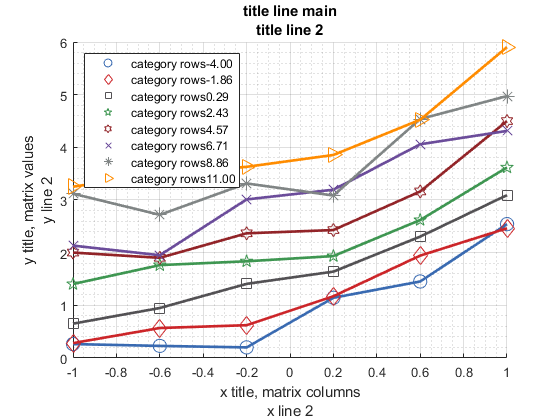
\includegraphics[width=5.20833in,height=\textheight]{img/fx_graph_grid_images/figure_0.png}

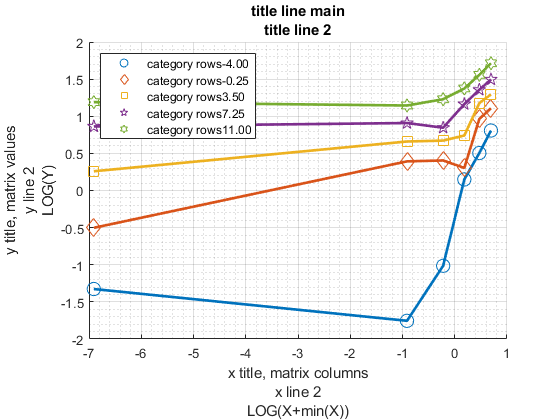
\includegraphics[width=5.20833in,height=\textheight]{img/fx_graph_grid_images/figure_1.png}

\hypertarget{test-ff_graph_grid-random-matrix-pick-markers-and-colors}{%
\subsection{Test FF\_GRAPH\_GRID Random Matrix Pick Markers and Colors}\label{test-ff_graph_grid-random-matrix-pick-markers-and-colors}}

Call the function with defaults.

\begin{verbatim}
rng(123);
mt_value = [normrnd(50,10,[1, 50]); ...
            normrnd(70,5,[1, 50]);...
            normrnd(90,10,[1, 50])];
ar_row_grid = ["shock low", "zero", "shock high"];
ar_col_grid = 1:50;
mp_support_graph = containers.Map('KeyType', 'char', 'ValueType', 'any');
mp_support_graph('cl_scatter_shapes') = { '.', 's' ,'.' };
mp_support_graph('cl_colors') = {'gray', 'red', 'gray'};
ff_graph_grid(mt_value, ar_row_grid, ar_col_grid, mp_support_graph);
\end{verbatim}

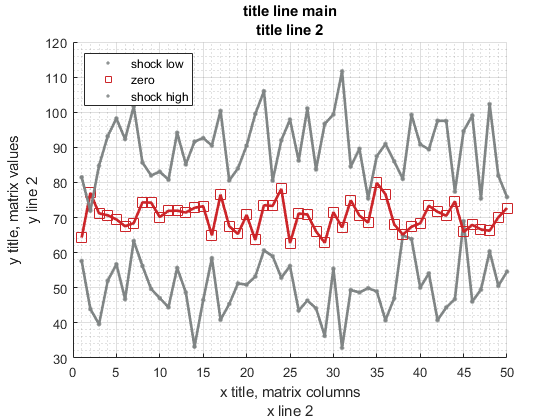
\includegraphics[width=5.20833in,height=\textheight]{img/fx_graph_grid_images/figure_2.png}

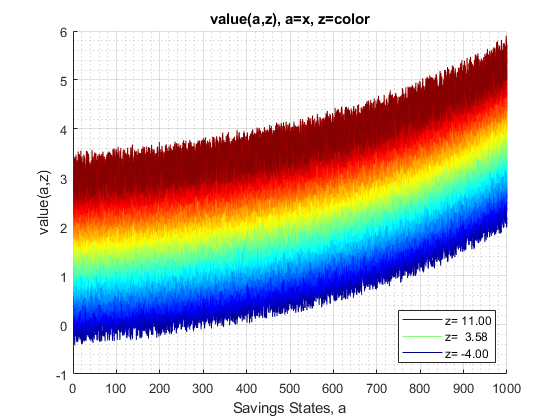
\includegraphics[width=5.20833in,height=\textheight]{img/fx_graph_grid_images/figure_3.png}

\hypertarget{test-ff_graph_grid-two-random-normal-lines-and-labels}{%
\subsection{Test FF\_GRAPH\_GRID Two Random Normal Lines and Labels}\label{test-ff_graph_grid-two-random-normal-lines-and-labels}}

There are two autoregressive time series, plot out the time two time
series.

\begin{verbatim}
% Generate the two time series
rng(456);
mt_value = normrnd(100,10,[2, 50]);
ar_row_grid = ["individual 1", "individual 2"];
ar_col_grid = 1:50;
mp_support_graph = containers.Map('KeyType', 'char', 'ValueType', 'any');
mp_support_graph('cl_st_graph_title') = {'Time Series Two Individuals'};
mp_support_graph('cl_st_ytitle') = {'Values'};
mp_support_graph('cl_st_xtitle') = {'Periods'};
mp_support_graph('bl_graph_logy') = false; % do not log
ff_graph_grid(mt_value, ar_row_grid, ar_col_grid, mp_support_graph);
\end{verbatim}

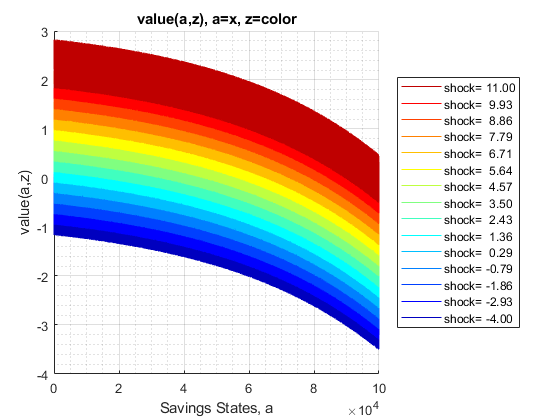
\includegraphics[width=5.20833in,height=\textheight]{img/fx_graph_grid_images/figure_4.png}

\hypertarget{test-ff_graph_grid-6-lines-pick-marker-and-colors}{%
\subsection{Test FF\_GRAPH\_GRID 6 Lines Pick Marker and Colors}\label{test-ff_graph_grid-6-lines-pick-marker-and-colors}}

Plot many lines, with auto legend.

\begin{verbatim}
% Generate some Data
rng(456);
ar_row_grid = linspace(-4, 11, 5);
ar_col_grid = linspace(-1, 1, 20);
rng(123);
mt_value = 0.2*ar_row_grid' + exp(ar_col_grid) + rand([length(ar_row_grid), length(ar_col_grid)]);
% container map settings
mp_support_graph = containers.Map('KeyType', 'char', 'ValueType', 'any');
mp_support_graph('cl_st_graph_title') = {'5 lines, specify marker and color, value(a,z), a=x, z=color'};
mp_support_graph('cl_st_ytitle') = {'value(a,z)'};
mp_support_graph('cl_st_xtitle') = {'Savings States, a'};
mp_support_graph('st_legend_loc') = 'southeast';
mp_support_graph('bl_graph_logy') = false; % do not log
mp_support_graph('st_rowvar_name') = 'z=';
mp_support_graph('it_legend_select') = 3; % how many shock legends to show
mp_support_graph('st_rounding') = '6.2f'; % format shock legend
mp_support_graph('cl_scatter_shapes') = {'s', 's', '*', '*', 'p'};
mp_support_graph('cl_colors') = {'green', 'black', 'green', 'black', 'orange'};
% Call function
ff_graph_grid(mt_value, ar_row_grid, ar_col_grid, mp_support_graph);
\end{verbatim}

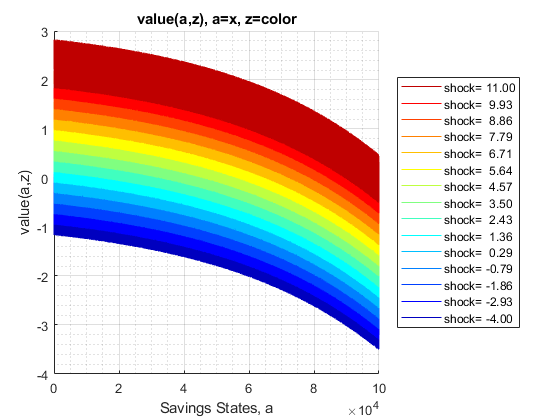
\includegraphics[width=5.20833in,height=\textheight]{img/fx_graph_grid_images/figure_5.png}

\hypertarget{test-ff_graph_grid-many-lines}{%
\subsection{Test FF\_GRAPH\_GRID Many Lines}\label{test-ff_graph_grid-many-lines}}

Plot many lines, with auto legend.

\begin{verbatim}
% Generate some Data
rng(456);
ar_row_grid = linspace(-4, 11, 100);
ar_col_grid = linspace(-1, 1, 1000);
rng(123);
mt_value = 0.2*ar_row_grid' + exp(ar_col_grid) + rand([length(ar_row_grid), length(ar_col_grid)]);
% container map settings
mp_support_graph = containers.Map('KeyType', 'char', 'ValueType', 'any');
mp_support_graph('cl_st_graph_title') = {'value(a,z), a=x, z=color'};
mp_support_graph('cl_st_ytitle') = {'value(a,z)'};
mp_support_graph('cl_st_xtitle') = {'Savings States, a'};
mp_support_graph('st_legend_loc') = 'southeast';
mp_support_graph('bl_graph_logy') = false; % do not log
mp_support_graph('st_rowvar_name') = 'z=';
mp_support_graph('it_legend_select') = 3; % how many shock legends to show
mp_support_graph('st_rounding') = '6.2f'; % format shock legend
mp_support_graph('cl_colors') = 'jet'; % any predefined matlab colormap
% Call function
ff_graph_grid(mt_value, ar_row_grid, ar_col_grid, mp_support_graph);
\end{verbatim}

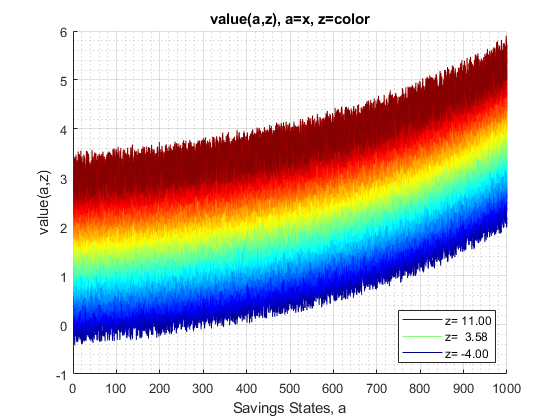
\includegraphics[width=5.20833in,height=\textheight]{img/fx_graph_grid_images/figure_6.png}

\hypertarget{test-ff_graph_grid-many-lines-legend-exogenous}{%
\subsection{Test FF\_GRAPH\_GRID Many Lines Legend Exogenous}\label{test-ff_graph_grid-many-lines-legend-exogenous}}

Plot many lines, exogenously set legend

\begin{verbatim}
% Generate the two time series
rng(456);
ar_row_grid = linspace(-4, 11, 15);
ar_col_grid = linspace(-1, 1, 100000);
rng(123);
mt_value = 0.2*ar_row_grid' - exp(ar_col_grid) + rand([length(ar_row_grid), length(ar_col_grid)]);
% setting shock vector name exogenously here
ar_row_grid = string(num2str(ar_row_grid', "shock=%6.2f"));
% container map settings
mp_support_graph = containers.Map('KeyType', 'char', 'ValueType', 'any');
mp_support_graph('cl_st_graph_title') = {'value(a,z), a=x, z=color'};
mp_support_graph('cl_st_ytitle') = {'value(a,z)'};
mp_support_graph('cl_st_xtitle') = {'Savings States, a'};
mp_support_graph('st_legend_loc') = 'eastoutside';
mp_support_graph('bl_graph_logy') = false; % do not log
mp_support_graph('it_legend_select') = 15;
mp_support_graph('cl_colors') = 'winter'; % any predefined matlab colormap
% Call function
ff_graph_grid(mt_value, ar_row_grid, ar_col_grid, mp_support_graph);
\end{verbatim}

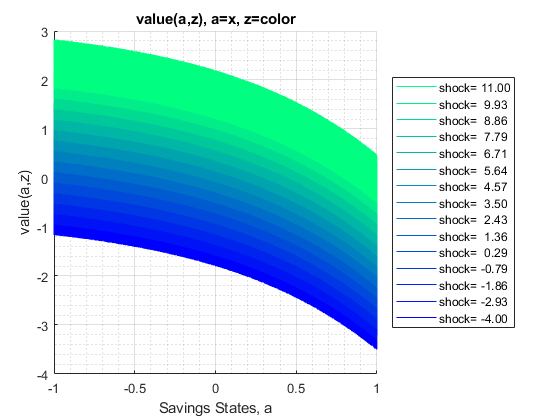
\includegraphics[width=5.20833in,height=\textheight]{img/fx_graph_grid_images/figure_7.png}

\hypertarget{data-structures}{%
\chapter{Data Structures}\label{data-structures}}

\hypertarget{ff_saveborr_grid-example-for-generating-asset-grid}{%
\section{FF\_SAVEBORR\_GRID Example for Generating Asset Grid}\label{ff_saveborr_grid-example-for-generating-asset-grid}}

\begin{quote}
Go back to \href{http://fanwangecon.github.io/}{fan}'s \href{https://fanwangecon.github.io/MEconTools/}{MEconTools} Toolbox (\href{https://fanwangecon.github.io/MEconTools/bookdown}{bookdown}), \href{https://fanwangecon.github.io/M4Econ/}{Matlab Code Examples} Repository (\href{https://fanwangecon.github.io/M4Econ/bookdown}{bookdown}), or \href{https://fanwangecon.github.io/Math4Econ/}{Math for Econ with Matlab} Repository (\href{https://fanwangecon.github.io/Math4Econ/bookdown}{bookdown}).
\end{quote}

This is the example vignette for function:
\href{https://github.com/FanWangEcon/MEconTools/blob/master/MEconTools/generate/ff_saveborr_grid.m}{\textbf{ff\_saveborr\_grid}}
from the \href{https://fanwangecon.github.io/MEconTools/}{\textbf{MEconTools
Package}}\textbf{.} This function
generates variously spaced savings/borrowing states/choices grid.

\hypertarget{test-ff_saveborr_grid-defaults}{%
\subsection{Test FF\_SAVEBORR\_GRID Defaults}\label{test-ff_saveborr_grid-defaults}}

Call the function with defaults.

\begin{verbatim}
ff_saveborr_grid();

----------------------------------------
xxxxxxxxxxxxxxxxxxxxxxxxxxxxxxxxxxxxxxxx
CONTAINER NAME: mp_container_map ND Array (Matrix etc)
xxxxxxxxxxxxxxxxxxxxxxxxxxxxxxxxxxxxxxxx
                      i    idx    ndim    numel    rowN    colN     sum     mean      std      coefvari    min    max
                      _    ___    ____    _____    ____    ____    _____    _____    ______    ________    ___    ___

    ar_fl_saveborr    1     1      2       25       25      1      216.7    8.668    13.363     1.5417      0     50 

xxx TABLE:ar_fl_saveborr xxxxxxxxxxxxxxxxxx
              c1   
           ________

    r1            0
    r2     0.029558
    r3     0.067855
    r4      0.11748
    r5      0.18177
    r6      0.26507
    r7      0.37301
    r8      0.51286
    r9      0.69407
    r10     0.92885
    r11      1.2331
    r12      1.6272
    r13      2.1379
    r14      2.7996
    r15       3.657
    r16      4.7679
    r17      6.2072
    r18      8.0722
    r19      10.489
    r20       13.62
    r21      17.676
    r22      22.932
    r23      29.743
    r24      38.567
    r25          50

----------------------------------------
xxxxxxxxxxxxxxxxxxxxxxxxxxxxxxxxxxxxxxxx
CONTAINER NAME: mp_container_map Scalars
xxxxxxxxxxxxxxxxxxxxxxxxxxxxxxxxxxxxxxxx
                              i    idx    value
                              _    ___    _____

    grid_evenlog_threshold    1     2        1 
    grid_log10space_x1        2     3      0.3 
    grid_log10space_x2        3     4        3 
    grid_powerspace_power     4     5        3 
\end{verbatim}

\hypertarget{test-ff_saveborr_grid-default-linear-grid-log-grid-power-grid-threshold-grid}{%
\subsection{Test FF\_SAVEBORR\_GRID Default Linear Grid, Log Grid, Power Grid, Threshold Grid}\label{test-ff_saveborr_grid-default-linear-grid-log-grid-power-grid-threshold-grid}}

Call the function with defaults.

\begin{verbatim}
% Same min and max and grid points
[fl_a_min, fl_a_max, it_a_points] = deal(0,50,25);
% Four types of grid points
st_grid_type = 'grid_linspace';
[ar_fl_saveborr_linspace] = ff_saveborr_grid(fl_a_min, fl_a_max, it_a_points, st_grid_type);
st_grid_type = 'grid_log10space';
[ar_fl_saveborr_log10space] = ff_saveborr_grid(fl_a_min, fl_a_max, it_a_points, st_grid_type);
st_grid_type = 'grid_powerspace';
[ar_fl_saveborr_powerspace] = ff_saveborr_grid(fl_a_min, fl_a_max, it_a_points, st_grid_type);
st_grid_type = 'grid_evenlog';
[ar_fl_saveborr_evenlog] = ff_saveborr_grid(fl_a_min, fl_a_max, it_a_points, st_grid_type);
% draw four types of lines jointly
mt_value = [ar_fl_saveborr_linspace'; ar_fl_saveborr_log10space'; ...
    ar_fl_saveborr_powerspace'; ar_fl_saveborr_evenlog'];
ar_row_grid = ["grid linspace", "grid log10space", "grid powerspace", "grid evenlog"];
ar_col_grid = 1:it_a_points;
mp_support_graph = containers.Map('KeyType', 'char', 'ValueType', 'any');
mp_support_graph('cl_st_graph_title') = {'Four Asset Grids with Default Parameters'};
mp_support_graph('cl_st_ytitle') = {'Asset Grid Points'};
mp_support_graph('cl_st_xtitle') = {'Asset Grid Counter'};
mp_support_graph('bl_graph_logy') = true; % do not log
ff_graph_grid(mt_value, ar_row_grid, ar_col_grid, mp_support_graph);
\end{verbatim}

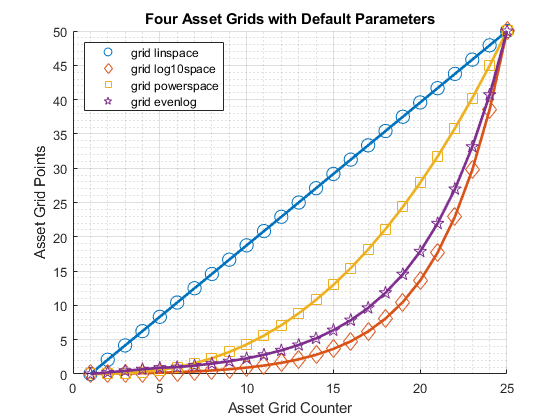
\includegraphics[width=5.20833in,height=\textheight]{img/fx_saveborr_grid_images/figure_0.png}

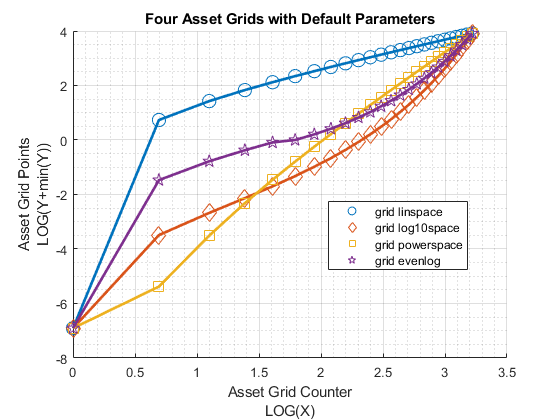
\includegraphics[width=5.20833in,height=\textheight]{img/fx_saveborr_grid_images/figure_1.png}

\hypertarget{test-ff_saveborr_grid-log-grid-changing-parameters}{%
\subsection{Test FF\_SAVEBORR\_GRID Log Grid Changing Parameters}\label{test-ff_saveborr_grid-log-grid-changing-parameters}}

Log grid, same min and max, change log X1 and X2 points

\begin{verbatim}
% Same min and max and grid points
[fl_a_min, fl_a_max, it_a_points] = deal(0,50,25);
st_grid_type = 'grid_log10space';
% Four types of grid points
mp_grid_control = containers.Map('KeyType','char', 'ValueType','any');
mp_grid_control('grid_log10space_x1') = 0.1;
mp_grid_control('grid_log10space_x2') = 1;
[ar_fl_log10space_a] = ff_saveborr_grid(fl_a_min, fl_a_max, it_a_points, st_grid_type, mp_grid_control);
mp_grid_control('grid_log10space_x1') = 0.1/2;
mp_grid_control('grid_log10space_x2') = 1*2;
[ar_fl_log10space_b] = ff_saveborr_grid(fl_a_min, fl_a_max, it_a_points, st_grid_type, mp_grid_control);
mp_grid_control('grid_log10space_x1') = 0.1/4;
mp_grid_control('grid_log10space_x2') = 1*4;
[ar_fl_log10space_c] = ff_saveborr_grid(fl_a_min, fl_a_max, it_a_points, st_grid_type, mp_grid_control);
mp_grid_control('grid_log10space_x1') = 0.1/6;
mp_grid_control('grid_log10space_x2') = 1*6;
[ar_fl_log10space_d] = ff_saveborr_grid(fl_a_min, fl_a_max, it_a_points, st_grid_type, mp_grid_control);
% draw four types of lines jointly
mt_value = [ar_fl_log10space_a'; ar_fl_log10space_b'; ...
    ar_fl_log10space_c'; ar_fl_log10space_d'];
ar_row_grid = [...
    "log10space:x1=0.1/1, x2=1", ...
    "log10space:x1=0.1/2, x2=2", ...
    "log10space:x1=0.1/4, x2=3", ...
    "log10space:x1=0.1/6, x2=4"];
ar_col_grid = 1:it_a_points;
mp_support_graph = containers.Map('KeyType', 'char', 'ValueType', 'any');
mp_support_graph('cl_st_graph_title') = {'Asset Grids with Log 10 Grid Varying Controls'};
mp_support_graph('cl_st_ytitle') = {'Asset Grid Points'};
mp_support_graph('cl_st_xtitle') = {'Asset Grid Counter'};
mp_support_graph('bl_graph_logy') = true; % do not log
ff_graph_grid(mt_value, ar_row_grid, ar_col_grid, mp_support_graph);
\end{verbatim}

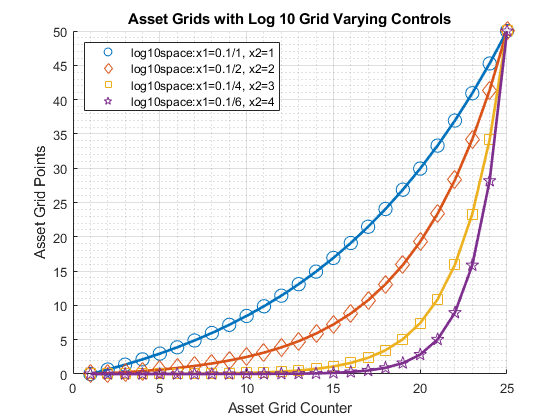
\includegraphics[width=5.20833in,height=\textheight]{img/fx_saveborr_grid_images/figure_2.png}

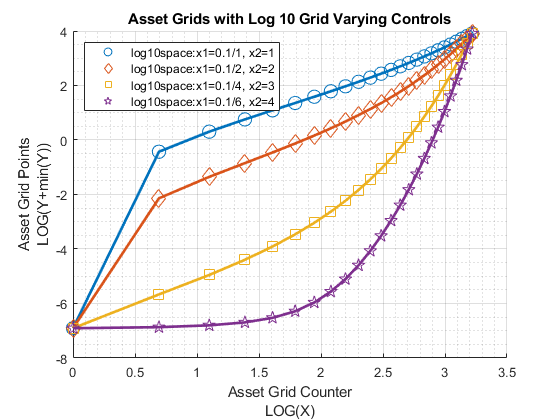
\includegraphics[width=5.20833in,height=\textheight]{img/fx_saveborr_grid_images/figure_3.png}

\hypertarget{test-ff_saveborr_grid-power-grid-changing-parameters}{%
\subsection{Test FF\_SAVEBORR\_GRID Power Grid Changing Parameters}\label{test-ff_saveborr_grid-power-grid-changing-parameters}}

Log grid, same min and max, change log X1 and X2 points

\begin{verbatim}
% Same min and max and grid points
[fl_a_min, fl_a_max, it_a_points] = deal(0,50,25);
st_grid_type = 'grid_powerspace';
% Four types of grid points
mp_grid_control = containers.Map('KeyType','char', 'ValueType','any');
mp_grid_control('grid_powerspace_power') = 1;
[ar_fl_powerspace_a] = ff_saveborr_grid(fl_a_min, fl_a_max, it_a_points, st_grid_type, mp_grid_control);
mp_grid_control('grid_powerspace_power') = 2;
[ar_fl_powerspace_b] = ff_saveborr_grid(fl_a_min, fl_a_max, it_a_points, st_grid_type, mp_grid_control);
mp_grid_control('grid_powerspace_power') = 4;
[ar_fl_powerspace_c] = ff_saveborr_grid(fl_a_min, fl_a_max, it_a_points, st_grid_type, mp_grid_control);
mp_grid_control('grid_powerspace_power') = 6;
[ar_fl_powerspace_d] = ff_saveborr_grid(fl_a_min, fl_a_max, it_a_points, st_grid_type, mp_grid_control);
% draw four types of lines jointly
mt_value = [ar_fl_powerspace_a'; ar_fl_powerspace_b'; ...
    ar_fl_powerspace_c'; ar_fl_powerspace_d'];
ar_row_grid = [...
    "powerspace:power=1", ...
    "powerspace:power=2", ...
    "powerspace:power=4", ...
    "powerspace:power=6"];
ar_col_grid = 1:it_a_points;
mp_support_graph = containers.Map('KeyType', 'char', 'ValueType', 'any');
mp_support_graph('cl_st_graph_title') = {'Asset Grids with Power Grid Varying Controls'};
mp_support_graph('cl_st_ytitle') = {'Asset Grid Points'};
mp_support_graph('cl_st_xtitle') = {'Asset Grid Counter'};
mp_support_graph('bl_graph_logy') = true; % do not log
ff_graph_grid(mt_value, ar_row_grid, ar_col_grid, mp_support_graph);
\end{verbatim}

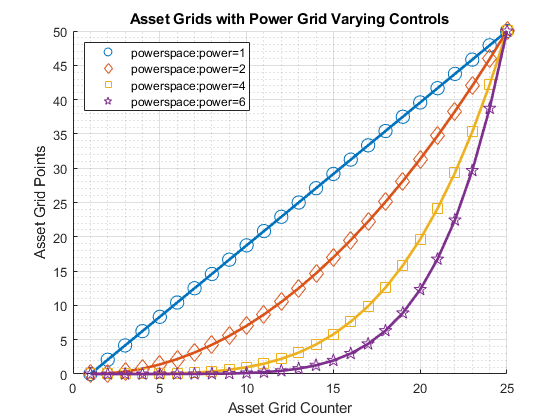
\includegraphics[width=5.20833in,height=\textheight]{img/fx_saveborr_grid_images/figure_4.png}

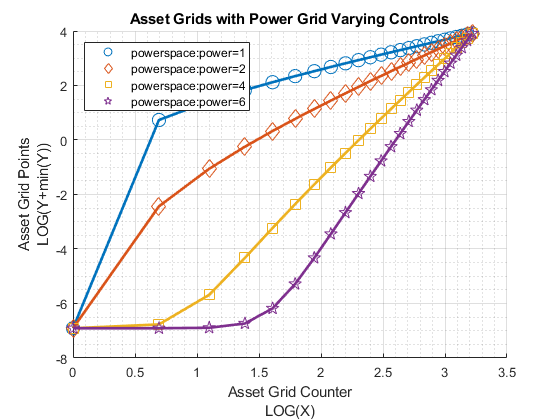
\includegraphics[width=5.20833in,height=\textheight]{img/fx_saveborr_grid_images/figure_5.png}

\hypertarget{test-ff_saveborr_grid-threshold-grid-changing-parameters}{%
\subsection{Test FF\_SAVEBORR\_GRID Threshold Grid Changing Parameters}\label{test-ff_saveborr_grid-threshold-grid-changing-parameters}}

Threshold Grid, Changing Threshold Levels. Initial segments below
threshold are linspace, then logspace.

\begin{verbatim}
% Same min and max and grid points
[fl_a_min, fl_a_max, it_a_points] = deal(0,50,25);
st_grid_type = 'grid_evenlog';
% Four types of grid points
mp_grid_control = containers.Map('KeyType','char', 'ValueType','any');
mp_grid_control('grid_evenlog_threshold') = 0.50;
[ar_fl_evenlog_a] = ff_saveborr_grid(fl_a_min, fl_a_max, it_a_points, st_grid_type, mp_grid_control);
mp_grid_control('grid_evenlog_threshold') = 1.00;
[ar_fl_evenlog_b] = ff_saveborr_grid(fl_a_min, fl_a_max, it_a_points, st_grid_type, mp_grid_control);
mp_grid_control('grid_evenlog_threshold') = 2;
[ar_fl_evenlog_c] = ff_saveborr_grid(fl_a_min, fl_a_max, it_a_points, st_grid_type, mp_grid_control);
mp_grid_control('grid_evenlog_threshold') = 5;
[ar_fl_evenlog_d] = ff_saveborr_grid(fl_a_min, fl_a_max, it_a_points, st_grid_type, mp_grid_control);
% draw four types of lines jointly
mt_value = [ar_fl_evenlog_a'; ar_fl_evenlog_b'; ...
    ar_fl_evenlog_c'; ar_fl_evenlog_d'];
ar_row_grid = [...
    "evenlog:threshold=0.5", ...
    "evenlog:threshold=1.0", ...
    "evenlog:threshold=2.0", ...
    "evenlog:threshold=5.0"];
ar_col_grid = 1:it_a_points;
mp_support_graph = containers.Map('KeyType', 'char', 'ValueType', 'any');
mp_support_graph('cl_st_graph_title') = {'Asset Grids with Threshold Grid Varying Controls'};
mp_support_graph('cl_st_ytitle') = {'Asset Grid Points'};
mp_support_graph('cl_st_xtitle') = {'Asset Grid Counter'};
mp_support_graph('bl_graph_logy') = true; % do not log
ff_graph_grid(mt_value, ar_row_grid, ar_col_grid, mp_support_graph);
\end{verbatim}

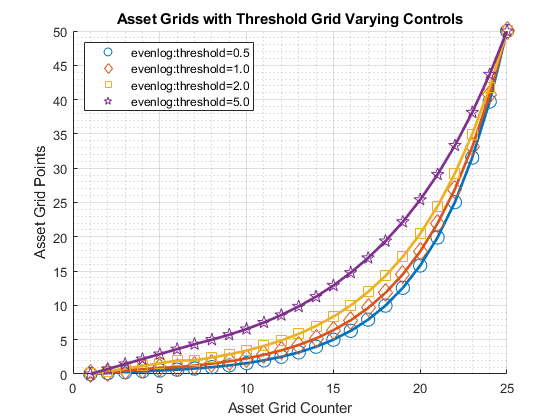
\includegraphics[width=5.20833in,height=\textheight]{img/fx_saveborr_grid_images/figure_6.png}

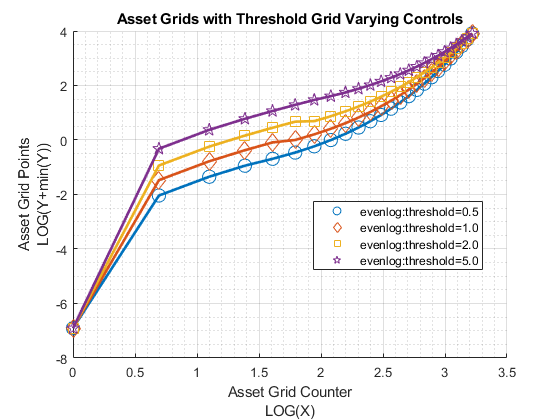
\includegraphics[width=5.20833in,height=\textheight]{img/fx_saveborr_grid_images/figure_7.png}

\hypertarget{common-functions}{%
\chapter{Common Functions}\label{common-functions}}

\hypertarget{ffy_tauchen-ar1-shock-discretization-example}{%
\section{FFY\_TAUCHEN AR1 Shock Discretization Example}\label{ffy_tauchen-ar1-shock-discretization-example}}

\begin{quote}
Go back to \href{http://fanwangecon.github.io/}{fan}'s \href{https://fanwangecon.github.io/MEconTools/}{MEconTools} Toolbox (\href{https://fanwangecon.github.io/MEconTools/bookdown}{bookdown}), \href{https://fanwangecon.github.io/M4Econ/}{Matlab Code Examples} Repository (\href{https://fanwangecon.github.io/M4Econ/bookdown}{bookdown}), or \href{https://fanwangecon.github.io/Math4Econ/}{Math for Econ with Matlab} Repository (\href{https://fanwangecon.github.io/Math4Econ/bookdown}{bookdown}).
\end{quote}

This is the example vignette for function:
\href{https://github.com/FanWangEcon/MEconTools/blob/master/MEconTools/external/stats/ffy_tauchen.m}{\textbf{ffy\_tauchen}}
from the \href{https://fanwangecon.github.io/MEconTools/}{\textbf{MEconTools
Package}}\textbf{.} : See also
the
\href{https://github.com/FanWangEcon/MEconTools/blob/master/MEconTools/external/stats/ffy_rouwenhorst.m}{\textbf{ffy\_rouwenhorst}}
function from the \href{https://fanwangecon.github.io/MEconTools/}{\textbf{MEconTools
Package}}\textbf{.} This function
discretize a mean zero AR1 process, uses Tauchen (1986). See \href{https://fanwangecon.github.io/M4Econ/panel/timeseries/htmlpdfm/fs_autoregressive.html}{AR 1
Example}
for some details on how the AR1 process works. And See \href{https://doi.org/10.1016/j.red.2010.02.002}{Kopecky and Suen
(2010)}.

\hypertarget{test-ffy_tauchen-defaults}{%
\subsection{Test FFY\_TAUCHEN Defaults}\label{test-ffy_tauchen-defaults}}

Call the function with defaults. Default sd bounds arer plus and minus
4. This is used in the following examples, unless otherwise specified as
the 5th parameter.

\begin{verbatim}
ffy_tauchen();

----------------------------------------
xxxxxxxxxxxxxxxxxxxxxxxxxxxxxxxxxxxxxxxx
CONTAINER NAME: mp_container_map ND Array (Matrix etc)
xxxxxxxxxxxxxxxxxxxxxxxxxxxxxxxxxxxxxxxx
                         i    idx    ndim    numel    rowN    colN    sum    mean      std      coefvari       min         max  
                         _    ___    ____    _____    ____    ____    ___    ____    _______    ________    __________    ______

    ar_disc_ar1          1     1      2        5       5       1       0       0     0.79057        Inf             -1         1
    mt_disc_ar1_trans    2     6      2       25       5       5       5     0.2     0.27623     1.3812     7.3923e-12    0.7887

xxx TABLE:ar_disc_ar1 xxxxxxxxxxxxxxxxxx
           c1 
          ____

    r1      -1
    r2    -0.5
    r3       0
    r4     0.5
    r5       1

xxx TABLE:mt_disc_ar1_trans xxxxxxxxxxxxxxxxxx
              c1            c2           c3           c4            c5    
          __________    __________    ________    __________    __________

    r1       0.22663       0.73331    0.040048    1.0689e-05    7.3923e-12
    r2      0.012224       0.58648     0.39831     0.0029797     7.605e-08
    r3    8.8417e-05       0.10556      0.7887       0.10556    8.8417e-05
    r4     7.605e-08     0.0029797     0.39831       0.58648      0.012224
    r5    7.3923e-12    1.0689e-05    0.040048       0.73331       0.22663

----------------------------------------
xxxxxxxxxxxxxxxxxxxxxxxxxxxxxxxxxxxxxxxx
CONTAINER NAME: mp_container_map Scalars
xxxxxxxxxxxxxxxxxxxxxxxxxxxxxxxxxxxxxxxx
                          i    idx    value
                          _    ___    _____

    fl_ar1_persistence    1     2      0.6 
    fl_ar1_step           2     3      0.5 
    fl_shk_std            3     4      0.2 
    it_std_bound          4     5        4 
\end{verbatim}

\hypertarget{test-ffy_tauchen-specify-parameters}{%
\subsection{Test FFY\_TAUCHEN Specify Parameters}\label{test-ffy_tauchen-specify-parameters}}

With a grid of 10 points, the sd bounds on Tauchen and Rouwenhorst are
identical. With the not extremely persistent shock process here, the
Tauchen and Rouwenhorst Results are very similar.

\begin{verbatim}
[fl_ar1_persistence, fl_shk_std, it_disc_points, bl_verbose, it_std_bound] = ...
    deal(0.60, 0.10, 10, true, 3);
ffy_tauchen(fl_ar1_persistence, fl_shk_std, it_disc_points, bl_verbose, it_std_bound);

----------------------------------------
xxxxxxxxxxxxxxxxxxxxxxxxxxxxxxxxxxxxxxxx
CONTAINER NAME: mp_container_map ND Array (Matrix etc)
xxxxxxxxxxxxxxxxxxxxxxxxxxxxxxxxxxxxxxxx
                         i    idx    ndim    numel    rowN    colN        sum           mean          std       coefvari         min          max  
                         _    ___    ____    _____    ____    ____    ___________    ___________    _______    ___________    __________    _______

    ar_disc_ar1          1     1      2        10      10       1     -7.2164e-16    -7.2164e-17     0.2523    -3.4962e+15        -0.375      0.375
    mt_disc_ar1_trans    2     6      2       100      10      10              10            0.1    0.11456         1.1456    1.1798e-08    0.32308

xxx TABLE:ar_disc_ar1 xxxxxxxxxxxxxxxxxx
              c1    
           _________

    r1        -0.375
    r2      -0.29167
    r3      -0.20833
    r4        -0.125
    r5     -0.041667
    r6      0.041667
    r7         0.125
    r8       0.20833
    r9       0.29167
    r10        0.375

xxx TABLE:mt_disc_ar1_trans xxxxxxxxxxxxxxxxxx
               c1            c2            c3            c4           c5          c6           c7            c8            c9           c10    
           __________    __________    __________    __________    ________    ________    __________    __________    __________    __________

    r1        0.13933       0.26196       0.31887       0.20154    0.066066    0.011201    0.00097859    4.3874e-05    1.0053e-06    1.1798e-08
    r2       0.056673       0.16995       0.30658       0.28713      0.1396    0.035167     0.0045756    0.00030628    1.0503e-05    1.8543e-07
    r3        0.01861      0.087039       0.23281       0.32308     0.23281    0.087039      0.016841     0.0016806    8.6129e-05    2.2881e-06
    r4      0.0048925      0.035167        0.1396       0.28713     0.30658     0.16995      0.048841     0.0072547    0.00055483    2.2197e-05
    r5      0.0010235      0.011201      0.066066       0.20154     0.31887     0.26196       0.11169       0.02466     0.0028101    0.00016962
    r6     0.00016962     0.0028101       0.02466       0.11169     0.26196     0.31887       0.20154      0.066066      0.011201     0.0010235
    r7     2.2197e-05    0.00055483     0.0072547      0.048841     0.16995     0.30658       0.28713        0.1396      0.035167     0.0048925
    r8     2.2881e-06    8.6129e-05     0.0016806      0.016841    0.087039     0.23281       0.32308       0.23281      0.087039       0.01861
    r9     1.8543e-07    1.0503e-05    0.00030628     0.0045756    0.035167      0.1396       0.28713       0.30658       0.16995      0.056673
    r10    1.1798e-08    1.0053e-06    4.3874e-05    0.00097859    0.011201    0.066066       0.20154       0.31887       0.26196       0.13933

----------------------------------------
xxxxxxxxxxxxxxxxxxxxxxxxxxxxxxxxxxxxxxxx
CONTAINER NAME: mp_container_map Scalars
xxxxxxxxxxxxxxxxxxxxxxxxxxxxxxxxxxxxxxxx
                          i    idx     value  
                          _    ___    ________

    fl_ar1_persistence    1     2          0.6
    fl_ar1_step           2     3     0.083333
    fl_shk_std            3     4          0.1
    it_std_bound          4     5            3
\end{verbatim}

\hypertarget{test-ffy_tauchen-high-persistence-low-sd}{%
\subsection{Test FFY\_TAUCHEN High Persistence, Low SD}\label{test-ffy_tauchen-high-persistence-low-sd}}

\begin{verbatim}
[fl_ar1_persistence, fl_shk_std, it_disc_points, bl_verbose] = ...
    deal(0.99, 0.01, 7, true);
ffy_tauchen(fl_ar1_persistence, fl_shk_std, it_disc_points, bl_verbose);

----------------------------------------
xxxxxxxxxxxxxxxxxxxxxxxxxxxxxxxxxxxxxxxx
CONTAINER NAME: mp_container_map ND Array (Matrix etc)
xxxxxxxxxxxxxxxxxxxxxxxxxxxxxxxxxxxxxxxx
                         i    idx    ndim    numel    rowN    colN        sum           mean          std       coefvari        min         max  
                         _    ___    ____    _____    ____    ____    ___________    ___________    _______    ___________    ________    _______

    ar_disc_ar1          1     1      2        7       7       1      -5.5511e-17    -7.9302e-18    0.20418    -2.5747e+16    -0.28355    0.28355
    mt_disc_ar1_trans    2     6      2       49       7       7                7        0.14286    0.35355         2.4749           0          1

xxx TABLE:ar_disc_ar1 xxxxxxxxxxxxxxxxxx
              c1     
          ___________

    r1       -0.28355
    r2       -0.18903
    r3      -0.094517
    r4    -2.7756e-17
    r5       0.094517
    r6        0.18903
    r7        0.28355

xxx TABLE:mt_disc_ar1_trans xxxxxxxxxxxxxxxxxx
              c1             c2             c3             c4             c5            c6            c7    
          ___________    ___________    ___________    ___________    __________    __________    __________

    r1              1     4.4497e-06              0              0             0             0             0
    r2     4.4412e-07              1     2.8552e-06              0             0             0             0
    r3      1.632e-46     7.1638e-07              1     1.8164e-06             0             0             0
    r4    9.6185e-124     6.3021e-46     1.1456e-06              1    1.1456e-06             0             0
    r5    6.3206e-239    8.9712e-123     2.4121e-45     1.8164e-06             1    7.1638e-07             0
    r6              0     1.426e-237    8.2932e-122     9.1503e-45    2.8552e-06             1    4.4412e-07
    r7              0              0    3.1885e-236    7.5984e-121    3.4405e-44    4.4497e-06             1

----------------------------------------
xxxxxxxxxxxxxxxxxxxxxxxxxxxxxxxxxxxxxxxx
CONTAINER NAME: mp_container_map Scalars
xxxxxxxxxxxxxxxxxxxxxxxxxxxxxxxxxxxxxxxx
                          i    idx     value  
                          _    ___    ________

    fl_ar1_persistence    1     2         0.99
    fl_ar1_step           2     3     0.094517
    fl_shk_std            3     4         0.01
    it_std_bound          4     5            4
\end{verbatim}

\hypertarget{test-ffy_tauchen-low-persistence-low-sd}{%
\subsection{Test FFY\_TAUCHEN Low Persistence, Low SD}\label{test-ffy_tauchen-low-persistence-low-sd}}

\begin{verbatim}
[fl_ar1_persistence, fl_shk_std, it_disc_points, bl_verbose] = ...
    deal(0.01, 0.01, 7, true);
ffy_tauchen(fl_ar1_persistence, fl_shk_std, it_disc_points, bl_verbose);

----------------------------------------
xxxxxxxxxxxxxxxxxxxxxxxxxxxxxxxxxxxxxxxx
CONTAINER NAME: mp_container_map ND Array (Matrix etc)
xxxxxxxxxxxxxxxxxxxxxxxxxxxxxxxxxxxxxxxx
                         i    idx    ndim    numel    rowN    colN    sum     mean        std       coefvari       min          max   
                         _    ___    ____    _____    ____    ____    ___    _______    ________    ________    __________    ________

    ar_disc_ar1          1     1      2        7       7       1       0           0    0.028805        Inf      -0.040002    0.040002
    mt_disc_ar1_trans    2     6      2       49       7       7       7     0.14286     0.17448     1.2213     0.00037109     0.49504

xxx TABLE:ar_disc_ar1 xxxxxxxxxxxxxxxxxx
             c1    
          _________

    r1    -0.040002
    r2    -0.026668
    r3    -0.013334
    r4            0
    r5     0.013334
    r6     0.026668
    r7     0.040002

xxx TABLE:mt_disc_ar1_trans xxxxxxxxxxxxxxxxxx
              c1           c2         c3         c4         c5          c6           c7    
          __________    ________    _______    _______    _______    ________    __________

    r1    0.00049475    0.024497    0.24044     0.4947    0.21921    0.020299    0.00037109
    r2    0.00047179    0.023751    0.23685    0.49488     0.2227    0.020954    0.00038948
    r3    0.00044982    0.023024    0.23329      0.495    0.22621    0.021626     0.0004087
    r4     0.0004288    0.022316    0.22974    0.49504    0.22974    0.022316     0.0004288
    r5     0.0004087    0.021626    0.22621      0.495    0.23329    0.023024    0.00044982
    r6    0.00038948    0.020954     0.2227    0.49488    0.23685    0.023751    0.00047179
    r7    0.00037109    0.020299    0.21921     0.4947    0.24044    0.024497    0.00049475

----------------------------------------
xxxxxxxxxxxxxxxxxxxxxxxxxxxxxxxxxxxxxxxx
CONTAINER NAME: mp_container_map Scalars
xxxxxxxxxxxxxxxxxxxxxxxxxxxxxxxxxxxxxxxx
                          i    idx     value  
                          _    ___    ________

    fl_ar1_persistence    1     2         0.01
    fl_ar1_step           2     3     0.013334
    fl_shk_std            3     4         0.01
    it_std_bound          4     5            4
\end{verbatim}

\hypertarget{test-ffy_tauchen-high-persistence-high-sd}{%
\subsection{Test FFY\_TAUCHEN High Persistence, High SD}\label{test-ffy_tauchen-high-persistence-high-sd}}

\begin{verbatim}
[fl_ar1_persistence, fl_shk_std, it_disc_points, bl_verbose] = ...
    deal(0.99, 0.99, 7, true);
ffy_tauchen(fl_ar1_persistence, fl_shk_std, it_disc_points, bl_verbose);

----------------------------------------
xxxxxxxxxxxxxxxxxxxxxxxxxxxxxxxxxxxxxxxx
CONTAINER NAME: mp_container_map ND Array (Matrix etc)
xxxxxxxxxxxxxxxxxxxxxxxxxxxxxxxxxxxxxxxx
                         i    idx    ndim    numel    rowN    colN        sum           mean          std       coefvari        min       max  
                         _    ___    ____    _____    ____    ____    ___________    ___________    _______    ___________    _______    ______

    ar_disc_ar1          1     1      2        7       7       1      -3.5527e-15    -5.0753e-16     20.214    -3.9828e+16    -28.072    28.072
    mt_disc_ar1_trans    2     6      2       49       7       7                7        0.14286    0.35355         2.4749          0         1

xxx TABLE:ar_disc_ar1 xxxxxxxxxxxxxxxxxx
            c1   
          _______

    r1    -28.072
    r2    -18.714
    r3    -9.3572
    r4          0
    r5     9.3572
    r6     18.714
    r7     28.072

xxx TABLE:mt_disc_ar1_trans xxxxxxxxxxxxxxxxxx
              c1             c2             c3             c4             c5            c6            c7    
          ___________    ___________    ___________    ___________    __________    __________    __________

    r1              1     4.4497e-06              0              0             0             0             0
    r2     4.4412e-07              1     2.8552e-06              0             0             0             0
    r3      1.632e-46     7.1638e-07              1     1.8164e-06             0             0             0
    r4    9.6185e-124     6.3021e-46     1.1456e-06              1    1.1456e-06             0             0
    r5    6.3206e-239    8.9712e-123     2.4121e-45     1.8164e-06             1    7.1638e-07             0
    r6              0     1.426e-237    8.2932e-122     9.1503e-45    2.8552e-06             1    4.4412e-07
    r7              0              0    3.1885e-236    7.5984e-121    3.4405e-44    4.4497e-06             1

----------------------------------------
xxxxxxxxxxxxxxxxxxxxxxxxxxxxxxxxxxxxxxxx
CONTAINER NAME: mp_container_map Scalars
xxxxxxxxxxxxxxxxxxxxxxxxxxxxxxxxxxxxxxxx
                          i    idx    value 
                          _    ___    ______

    fl_ar1_persistence    1     2       0.99
    fl_ar1_step           2     3     9.3572
    fl_shk_std            3     4       0.99
    it_std_bound          4     5          4
\end{verbatim}

\hypertarget{test-ffy_tauchen-low-persistence-low-sd-1}{%
\subsection{Test FFY\_TAUCHEN Low Persistence, Low SD}\label{test-ffy_tauchen-low-persistence-low-sd-1}}

\begin{verbatim}
[fl_ar1_persistence, fl_shk_std, it_disc_points, bl_verbose] = ...
    deal(0.01, 0.01, 7, true);
ffy_tauchen(fl_ar1_persistence, fl_shk_std, it_disc_points, bl_verbose);

----------------------------------------
xxxxxxxxxxxxxxxxxxxxxxxxxxxxxxxxxxxxxxxx
CONTAINER NAME: mp_container_map ND Array (Matrix etc)
xxxxxxxxxxxxxxxxxxxxxxxxxxxxxxxxxxxxxxxx
                         i    idx    ndim    numel    rowN    colN    sum     mean        std       coefvari       min          max   
                         _    ___    ____    _____    ____    ____    ___    _______    ________    ________    __________    ________

    ar_disc_ar1          1     1      2        7       7       1       0           0    0.028805        Inf      -0.040002    0.040002
    mt_disc_ar1_trans    2     6      2       49       7       7       7     0.14286     0.17448     1.2213     0.00037109     0.49504

xxx TABLE:ar_disc_ar1 xxxxxxxxxxxxxxxxxx
             c1    
          _________

    r1    -0.040002
    r2    -0.026668
    r3    -0.013334
    r4            0
    r5     0.013334
    r6     0.026668
    r7     0.040002

xxx TABLE:mt_disc_ar1_trans xxxxxxxxxxxxxxxxxx
              c1           c2         c3         c4         c5          c6           c7    
          __________    ________    _______    _______    _______    ________    __________

    r1    0.00049475    0.024497    0.24044     0.4947    0.21921    0.020299    0.00037109
    r2    0.00047179    0.023751    0.23685    0.49488     0.2227    0.020954    0.00038948
    r3    0.00044982    0.023024    0.23329      0.495    0.22621    0.021626     0.0004087
    r4     0.0004288    0.022316    0.22974    0.49504    0.22974    0.022316     0.0004288
    r5     0.0004087    0.021626    0.22621      0.495    0.23329    0.023024    0.00044982
    r6    0.00038948    0.020954     0.2227    0.49488    0.23685    0.023751    0.00047179
    r7    0.00037109    0.020299    0.21921     0.4947    0.24044    0.024497    0.00049475

----------------------------------------
xxxxxxxxxxxxxxxxxxxxxxxxxxxxxxxxxxxxxxxx
CONTAINER NAME: mp_container_map Scalars
xxxxxxxxxxxxxxxxxxxxxxxxxxxxxxxxxxxxxxxx
                          i    idx     value  
                          _    ___    ________

    fl_ar1_persistence    1     2         0.01
    fl_ar1_step           2     3     0.013334
    fl_shk_std            3     4         0.01
    it_std_bound          4     5            4
\end{verbatim}

\hypertarget{ffy_rouwenhorst-ar1-shock-discretization-example}{%
\section{FFY\_ROUWENHORST AR1 Shock Discretization Example}\label{ffy_rouwenhorst-ar1-shock-discretization-example}}

\begin{quote}
Go back to \href{http://fanwangecon.github.io/}{fan}'s \href{https://fanwangecon.github.io/MEconTools/}{MEconTools} Toolbox (\href{https://fanwangecon.github.io/MEconTools/bookdown}{bookdown}), \href{https://fanwangecon.github.io/M4Econ/}{Matlab Code Examples} Repository (\href{https://fanwangecon.github.io/M4Econ/bookdown}{bookdown}), or \href{https://fanwangecon.github.io/Math4Econ/}{Math for Econ with Matlab} Repository (\href{https://fanwangecon.github.io/Math4Econ/bookdown}{bookdown}).
\end{quote}

This is the example vignette for function:
\href{https://github.com/FanWangEcon/MEconTools/blob/master/MEconTools/external/stats/ffy_rouwenhorst.m}{\textbf{ffy\_rouwenhorst}}
from the \href{https://fanwangecon.github.io/MEconTools/}{\textbf{MEconTools
Package}}\textbf{.} See also
\href{https://github.com/FanWangEcon/MEconTools/blob/master/MEconTools/external/stats/ffy_tauchen.m}{\textbf{ffy\_tauchen}}
function from the \href{https://fanwangecon.github.io/MEconTools/}{\textbf{MEconTools
Package}}\textbf{.} This function
discretize a mean zero AR1 process, uses Rouwenhorst (1995). See \href{https://fanwangecon.github.io/M4Econ/panel/timeseries/htmlpdfm/fs_autoregressive.html}{AR 1
Example}
for some details on how the AR1 process works. And See \href{https://doi.org/10.1016/j.red.2010.02.002}{Kopecky and Suen
(2010)}.

\hypertarget{test-ffy_rouwenhorst-defaults}{%
\subsection{Test FFY\_ROUWENHORST Defaults}\label{test-ffy_rouwenhorst-defaults}}

Call the function with defaults.

\begin{verbatim}
ffy_rouwenhorst();

----------------------------------------
xxxxxxxxxxxxxxxxxxxxxxxxxxxxxxxxxxxxxxxx
CONTAINER NAME: mp_container_map ND Array (Matrix etc)
xxxxxxxxxxxxxxxxxxxxxxxxxxxxxxxxxxxxxxxx
                         i    idx    ndim    numel    rowN    colN    sum    mean      std      coefvari     min       max  
                         _    ___    ____    _____    ____    ____    ___    ____    _______    ________    ______    ______

    ar_disc_ar1          1     1      2        5       5       1       0       0     0.39528        Inf       -0.5       0.5
    mt_disc_ar1_trans    2    11      2       25       5       5       5     0.2     0.18246    0.91229     0.0016    0.5136

xxx TABLE:ar_disc_ar1 xxxxxxxxxxxxxxxxxx
           c1  
          _____

    r1     -0.5
    r2    -0.25
    r3        0
    r4     0.25
    r5      0.5

xxx TABLE:mt_disc_ar1_trans xxxxxxxxxxxxxxxxxx
            c1        c2        c3        c4        c5  
          ______    ______    ______    ______    ______

    r1    0.4096    0.4096    0.1536    0.0256    0.0016
    r2    0.1024    0.4864    0.3264    0.0784    0.0064
    r3    0.0256    0.2176    0.5136    0.2176    0.0256
    r4    0.0064    0.0784    0.3264    0.4864    0.1024
    r5    0.0016    0.0256    0.1536    0.4096    0.4096

----------------------------------------
xxxxxxxxxxxxxxxxxxxxxxxxxxxxxxxxxxxxxxxx
CONTAINER NAME: mp_container_map Scalars
xxxxxxxxxxxxxxxxxxxxxxxxxxxxxxxxxxxxxxxx
                          i    idx    value
                          _    ___    _____

    fl_ar1_beg            1     2     -0.5 
    fl_ar1_end            2     3      0.5 
    fl_ar1_persistence    3     4      0.6 
    fl_ar1_step           4     5     0.25 
    fl_p0                 5     6      0.8 
    fl_q0                 6     7      0.8 
    fl_shk_std            7     8      0.2 
    fl_sig_ar1            8     9     0.25 
    it_std_bound          9    10        0 
\end{verbatim}

\hypertarget{test-ffy_rouwenhorst-specify-parameters}{%
\subsection{Test FFY\_ROUWENHORST Specify Parameters}\label{test-ffy_rouwenhorst-specify-parameters}}

With a grid of 10 points, the Rwouenhorst bounds on standard deviations
are equall to Tauchen bounds of 3. With the not extremely persistent
shock process here, the Tauchen and Rouwenhorst Results are very
similar.

\begin{verbatim}
[fl_ar1_persistence, fl_shk_std, it_disc_points, bl_verbose] = ...
    deal(0.60, 0.10, 10, true);
ffy_rouwenhorst(fl_ar1_persistence, fl_shk_std, it_disc_points, bl_verbose);

----------------------------------------
xxxxxxxxxxxxxxxxxxxxxxxxxxxxxxxxxxxxxxxx
CONTAINER NAME: mp_container_map ND Array (Matrix etc)
xxxxxxxxxxxxxxxxxxxxxxxxxxxxxxxxxxxxxxxx
                         i    idx    ndim    numel    rowN    colN       sum           mean         std       coefvari       min         max  
                         _    ___    ____    _____    ____    ____    __________    __________    _______    __________    ________    _______

    ar_disc_ar1          1     1      2        10      10       1     5.5511e-17    5.5511e-18     0.2523    4.5451e+16      -0.375      0.375
    mt_disc_ar1_trans    2    11      2       100      10      10             10           0.1    0.11724        1.1724    5.12e-07    0.33477

xxx TABLE:ar_disc_ar1 xxxxxxxxxxxxxxxxxx
              c1    
           _________

    r1        -0.375
    r2      -0.29167
    r3      -0.20833
    r4        -0.125
    r5     -0.041667
    r6      0.041667
    r7         0.125
    r8       0.20833
    r9       0.29167
    r10        0.375

xxx TABLE:mt_disc_ar1_trans xxxxxxxxxxxxxxxxxx
               c1            c2            c3           c4           c5          c6          c7            c8            c9           c10    
           __________    __________    __________    _________    ________    ________    _________    __________    __________    __________

    r1        0.13422       0.30199       0.30199      0.17616     0.06606    0.016515    0.0027525    0.00029491    1.8432e-05      5.12e-07
    r2       0.033554       0.20133       0.32716      0.26424     0.12662    0.038535    0.0075694    0.00093389    6.6048e-05     2.048e-06
    r3      0.0083886      0.081789       0.26267      0.32755     0.21401    0.082747     0.019741     0.0028677    0.00023347     8.192e-06
    r4      0.0020972      0.028312       0.14038      0.30946     0.30369     0.15877     0.047989     0.0084603    0.00081101    3.2768e-05
    r5     0.00052429      0.009044      0.061145      0.20246     0.33477     0.25969      0.10585      0.023642     0.0027525    0.00013107
    r6     0.00013107     0.0027525      0.023642      0.10585     0.25969     0.33477      0.20246      0.061145      0.009044    0.00052429
    r7     3.2768e-05    0.00081101     0.0084603     0.047989     0.15877     0.30369      0.30946       0.14038      0.028312     0.0020972
    r8      8.192e-06    0.00023347     0.0028677     0.019741    0.082747     0.21401      0.32755       0.26267      0.081789     0.0083886
    r9      2.048e-06    6.6048e-05    0.00093389    0.0075694    0.038535     0.12662      0.26424       0.32716       0.20133      0.033554
    r10      5.12e-07    1.8432e-05    0.00029491    0.0027525    0.016515     0.06606      0.17616       0.30199       0.30199       0.13422

----------------------------------------
xxxxxxxxxxxxxxxxxxxxxxxxxxxxxxxxxxxxxxxx
CONTAINER NAME: mp_container_map Scalars
xxxxxxxxxxxxxxxxxxxxxxxxxxxxxxxxxxxxxxxx
                          i    idx     value  
                          _    ___    ________

    fl_ar1_beg            1     2       -0.375
    fl_ar1_end            2     3        0.375
    fl_ar1_persistence    3     4          0.6
    fl_ar1_step           4     5     0.083333
    fl_p0                 5     6          0.8
    fl_q0                 6     7          0.8
    fl_shk_std            7     8          0.1
    fl_sig_ar1            8     9        0.125
    it_std_bound          9    10            0
\end{verbatim}

\hypertarget{test-ffy_rouwenhorst-high-persistence-low-sd}{%
\subsection{Test FFY\_ROUWENHORST High Persistence, Low SD}\label{test-ffy_rouwenhorst-high-persistence-low-sd}}

\begin{verbatim}
[fl_ar1_persistence, fl_shk_std, it_disc_points, bl_verbose] = ...
    deal(0.99, 0.01, 7, true);
ffy_rouwenhorst(fl_ar1_persistence, fl_shk_std, it_disc_points, bl_verbose);

----------------------------------------
xxxxxxxxxxxxxxxxxxxxxxxxxxxxxxxxxxxxxxxx
CONTAINER NAME: mp_container_map ND Array (Matrix etc)
xxxxxxxxxxxxxxxxxxxxxxxxxxxxxxxxxxxxxxxx
                         i    idx    ndim    numel    rowN    colN    sum     mean        std      coefvari       min          max  
                         _    ___    ____    _____    ____    ____    ___    _______    _______    ________    __________    _______

    ar_disc_ar1          1     1      2        7       7       1       0           0    0.12503        Inf       -0.17364    0.17364
    mt_disc_ar1_trans    2    11      2       49       7       7       7     0.14286    0.34148     2.3904     1.5625e-14    0.97059

xxx TABLE:ar_disc_ar1 xxxxxxxxxxxxxxxxxx
             c1   
          ________

    r1    -0.17364
    r2    -0.11576
    r3    -0.05788
    r4           0
    r5     0.05788
    r6     0.11576
    r7     0.17364

xxx TABLE:mt_disc_ar1_trans xxxxxxxxxxxxxxxxxx
              c1            c2            c3            c4            c5            c6            c7    
          __________    __________    __________    __________    __________    __________    __________

    r1       0.97037      0.029257    0.00036756    2.4627e-06    9.2815e-09    1.8656e-11    1.5625e-14
    r2     0.0048762        0.9705      0.024382    0.00024504    1.2314e-06    3.0938e-09    3.1094e-12
    r3    2.4504e-05      0.009753       0.97057      0.019506    0.00014703    4.9254e-07    6.1877e-10
    r4    1.2313e-07    7.3513e-05       0.01463       0.97059       0.01463    7.3513e-05    1.2313e-07
    r5    6.1877e-10    4.9254e-07    0.00014703      0.019506       0.97057      0.009753    2.4504e-05
    r6    3.1094e-12    3.0938e-09    1.2314e-06    0.00024504      0.024382        0.9705     0.0048762
    r7    1.5625e-14    1.8656e-11    9.2815e-09    2.4627e-06    0.00036756      0.029257       0.97037

----------------------------------------
xxxxxxxxxxxxxxxxxxxxxxxxxxxxxxxxxxxxxxxx
CONTAINER NAME: mp_container_map Scalars
xxxxxxxxxxxxxxxxxxxxxxxxxxxxxxxxxxxxxxxx
                          i    idx     value  
                          _    ___    ________

    fl_ar1_beg            1     2     -0.17364
    fl_ar1_end            2     3      0.17364
    fl_ar1_persistence    3     4         0.99
    fl_ar1_step           4     5      0.05788
    fl_p0                 5     6        0.995
    fl_q0                 6     7        0.995
    fl_shk_std            7     8         0.01
    fl_sig_ar1            8     9     0.070888
    it_std_bound          9    10            0
\end{verbatim}

\hypertarget{test-ffy_rouwenhorst-low-persistence-low-sd}{%
\subsection{Test FFY\_ROUWENHORST Low Persistence, Low SD}\label{test-ffy_rouwenhorst-low-persistence-low-sd}}

\begin{verbatim}
[fl_ar1_persistence, fl_shk_std, it_disc_points, bl_verbose] = ...
    deal(0.01, 0.01, 7, true);
ffy_rouwenhorst(fl_ar1_persistence, fl_shk_std, it_disc_points, bl_verbose);

----------------------------------------
xxxxxxxxxxxxxxxxxxxxxxxxxxxxxxxxxxxxxxxx
CONTAINER NAME: mp_container_map ND Array (Matrix etc)
xxxxxxxxxxxxxxxxxxxxxxxxxxxxxxxxxxxxxxxx
                         i    idx    ndim    numel    rowN    colN    sum     mean        std       coefvari       min         max   
                         _    ___    ____    _____    ____    ____    ___    _______    ________    ________    _________    ________

    ar_disc_ar1          1     1      2        7       7       1       0           0    0.017639        Inf     -0.024496    0.024496
    mt_disc_ar1_trans    2    11      2       49       7       7       7     0.14286     0.10985    0.76893      0.014711     0.31252

xxx TABLE:ar_disc_ar1 xxxxxxxxxxxxxxxxxx
              c1    
          __________

    r1     -0.024496
    r2     -0.016331
    r3    -0.0081654
    r4             0
    r5     0.0081654
    r6      0.016331
    r7      0.024496

xxx TABLE:mt_disc_ar1_trans xxxxxxxxxxxxxxxxxx
             c1          c2         c3         c4         c5          c6          c7   
          ________    ________    _______    _______    _______    ________    ________

    r1    0.016586    0.097547    0.23904    0.31241    0.22966    0.090047    0.014711
    r2    0.016258    0.096266    0.23749    0.31247    0.23124    0.091266    0.015008
    r3    0.015936    0.094997    0.23594    0.31251    0.23281    0.092497    0.015311
    r4     0.01562    0.093741    0.23438    0.31252    0.23438    0.093741     0.01562
    r5    0.015311    0.092497    0.23281    0.31251    0.23594    0.094997    0.015936
    r6    0.015008    0.091266    0.23124    0.31247    0.23749    0.096266    0.016258
    r7    0.014711    0.090047    0.22966    0.31241    0.23904    0.097547    0.016586

----------------------------------------
xxxxxxxxxxxxxxxxxxxxxxxxxxxxxxxxxxxxxxxx
CONTAINER NAME: mp_container_map Scalars
xxxxxxxxxxxxxxxxxxxxxxxxxxxxxxxxxxxxxxxx
                          i    idx      value  
                          _    ___    _________

    fl_ar1_beg            1     2     -0.024496
    fl_ar1_end            2     3      0.024496
    fl_ar1_persistence    3     4          0.01
    fl_ar1_step           4     5     0.0081654
    fl_p0                 5     6         0.505
    fl_q0                 6     7         0.505
    fl_shk_std            7     8          0.01
    fl_sig_ar1            8     9      0.010001
    it_std_bound          9    10             0
\end{verbatim}

\hypertarget{test-ffy_rouwenhorst-high-persistence-high-sd}{%
\subsection{Test FFY\_ROUWENHORST High Persistence, High SD}\label{test-ffy_rouwenhorst-high-persistence-high-sd}}

\begin{verbatim}
[fl_ar1_persistence, fl_shk_std, it_disc_points, bl_verbose] = ...
    deal(0.99, 0.99, 7, true);
ffy_rouwenhorst(fl_ar1_persistence, fl_shk_std, it_disc_points, bl_verbose);

----------------------------------------
xxxxxxxxxxxxxxxxxxxxxxxxxxxxxxxxxxxxxxxx
CONTAINER NAME: mp_container_map ND Array (Matrix etc)
xxxxxxxxxxxxxxxxxxxxxxxxxxxxxxxxxxxxxxxx
                         i    idx    ndim    numel    rowN    colN       sum           mean         std      coefvari        min          max  
                         _    ___    ____    _____    ____    ____    __________    __________    _______    _________    __________    _______

    ar_disc_ar1          1     1      2        7       7       1      3.5527e-15    5.0753e-16     12.378    2.439e+16        -17.19      17.19
    mt_disc_ar1_trans    2    11      2       49       7       7               7       0.14286    0.34148       2.3904    1.5625e-14    0.97059

xxx TABLE:ar_disc_ar1 xxxxxxxxxxxxxxxxxx
            c1   
          _______

    r1     -17.19
    r2     -11.46
    r3    -5.7301
    r4          0
    r5     5.7301
    r6      11.46
    r7      17.19

xxx TABLE:mt_disc_ar1_trans xxxxxxxxxxxxxxxxxx
              c1            c2            c3            c4            c5            c6            c7    
          __________    __________    __________    __________    __________    __________    __________

    r1       0.97037      0.029257    0.00036756    2.4627e-06    9.2815e-09    1.8656e-11    1.5625e-14
    r2     0.0048762        0.9705      0.024382    0.00024504    1.2314e-06    3.0938e-09    3.1094e-12
    r3    2.4504e-05      0.009753       0.97057      0.019506    0.00014703    4.9254e-07    6.1877e-10
    r4    1.2313e-07    7.3513e-05       0.01463       0.97059       0.01463    7.3513e-05    1.2313e-07
    r5    6.1877e-10    4.9254e-07    0.00014703      0.019506       0.97057      0.009753    2.4504e-05
    r6    3.1094e-12    3.0938e-09    1.2314e-06    0.00024504      0.024382        0.9705     0.0048762
    r7    1.5625e-14    1.8656e-11    9.2815e-09    2.4627e-06    0.00036756      0.029257       0.97037

----------------------------------------
xxxxxxxxxxxxxxxxxxxxxxxxxxxxxxxxxxxxxxxx
CONTAINER NAME: mp_container_map Scalars
xxxxxxxxxxxxxxxxxxxxxxxxxxxxxxxxxxxxxxxx
                          i    idx    value 
                          _    ___    ______

    fl_ar1_beg            1     2     -17.19
    fl_ar1_end            2     3      17.19
    fl_ar1_persistence    3     4       0.99
    fl_ar1_step           4     5     5.7301
    fl_p0                 5     6      0.995
    fl_q0                 6     7      0.995
    fl_shk_std            7     8       0.99
    fl_sig_ar1            8     9     7.0179
    it_std_bound          9    10          0
\end{verbatim}

\hypertarget{test-ffy_rouwenhorst-low-persistence-low-sd-1}{%
\subsection{Test FFY\_ROUWENHORST Low Persistence, Low SD}\label{test-ffy_rouwenhorst-low-persistence-low-sd-1}}

\begin{verbatim}
[fl_ar1_persistence, fl_shk_std, it_disc_points, bl_verbose] = ...
    deal(0.01, 0.01, 7, true);
ffy_rouwenhorst(fl_ar1_persistence, fl_shk_std, it_disc_points, bl_verbose);

----------------------------------------
xxxxxxxxxxxxxxxxxxxxxxxxxxxxxxxxxxxxxxxx
CONTAINER NAME: mp_container_map ND Array (Matrix etc)
xxxxxxxxxxxxxxxxxxxxxxxxxxxxxxxxxxxxxxxx
                         i    idx    ndim    numel    rowN    colN    sum     mean        std       coefvari       min         max   
                         _    ___    ____    _____    ____    ____    ___    _______    ________    ________    _________    ________

    ar_disc_ar1          1     1      2        7       7       1       0           0    0.017639        Inf     -0.024496    0.024496
    mt_disc_ar1_trans    2    11      2       49       7       7       7     0.14286     0.10985    0.76893      0.014711     0.31252

xxx TABLE:ar_disc_ar1 xxxxxxxxxxxxxxxxxx
              c1    
          __________

    r1     -0.024496
    r2     -0.016331
    r3    -0.0081654
    r4             0
    r5     0.0081654
    r6      0.016331
    r7      0.024496

xxx TABLE:mt_disc_ar1_trans xxxxxxxxxxxxxxxxxx
             c1          c2         c3         c4         c5          c6          c7   
          ________    ________    _______    _______    _______    ________    ________

    r1    0.016586    0.097547    0.23904    0.31241    0.22966    0.090047    0.014711
    r2    0.016258    0.096266    0.23749    0.31247    0.23124    0.091266    0.015008
    r3    0.015936    0.094997    0.23594    0.31251    0.23281    0.092497    0.015311
    r4     0.01562    0.093741    0.23438    0.31252    0.23438    0.093741     0.01562
    r5    0.015311    0.092497    0.23281    0.31251    0.23594    0.094997    0.015936
    r6    0.015008    0.091266    0.23124    0.31247    0.23749    0.096266    0.016258
    r7    0.014711    0.090047    0.22966    0.31241    0.23904    0.097547    0.016586

----------------------------------------
xxxxxxxxxxxxxxxxxxxxxxxxxxxxxxxxxxxxxxxx
CONTAINER NAME: mp_container_map Scalars
xxxxxxxxxxxxxxxxxxxxxxxxxxxxxxxxxxxxxxxx
                          i    idx      value  
                          _    ___    _________

    fl_ar1_beg            1     2     -0.024496
    fl_ar1_end            2     3      0.024496
    fl_ar1_persistence    3     4          0.01
    fl_ar1_step           4     5     0.0081654
    fl_p0                 5     6         0.505
    fl_q0                 6     7         0.505
    fl_shk_std            7     8          0.01
    fl_sig_ar1            8     9      0.010001
    it_std_bound          9    10             0
\end{verbatim}

\hypertarget{support-tools}{%
\chapter{Support Tools}\label{support-tools}}

\hypertarget{ff_container_map_display-examples}{%
\section{FF\_CONTAINER\_MAP\_DISPLAY Examples}\label{ff_container_map_display-examples}}

\begin{quote}
Go back to \href{http://fanwangecon.github.io/}{fan}'s \href{https://fanwangecon.github.io/MEconTools/}{MEconTools} Toolbox (\href{https://fanwangecon.github.io/MEconTools/bookdown}{bookdown}), \href{https://fanwangecon.github.io/M4Econ/}{Matlab Code Examples} Repository (\href{https://fanwangecon.github.io/M4Econ/bookdown}{bookdown}), or \href{https://fanwangecon.github.io/Math4Econ/}{Math for Econ with Matlab} Repository (\href{https://fanwangecon.github.io/Math4Econ/bookdown}{bookdown}).
\end{quote}

This is the example vignette for function:
\href{https://github.com/FanWangEcon/MEconTools/blob/master/MEconTools/tools/ff_container_map_display.m}{\textbf{ff\_container\_map\_display}}
from the \href{https://fanwangecon.github.io/MEconTools/}{\textbf{MEconTools
Package}}\textbf{.} This function
summarizes statistics of matrixes stored in a container map, as well as
scalar, string, function and other values stored in container maps.

\hypertarget{test-ff_container_map_display-defaults}{%
\subsection{Test FF\_CONTAINER\_MAP\_DISPLAY Defaults}\label{test-ff_container_map_display-defaults}}

Call the function with defaults.

\begin{verbatim}
ff_container_map_display();

----------------------------------------
xxxxxxxxxxxxxxxxxxxxxxxxxxxxxxxxxxxxxxxx
 ND Array (Matrix etc)
xxxxxxxxxxxxxxxxxxxxxxxxxxxxxxxxxxxxxxxx
                      i     idx    ndim    numel    rowN    colN     sum       mean        std      coefvari       min          max  
                      __    ___    ____    _____    ____    ____    ______    _______    _______    ________    __________    _______

    mat_1              1     7      2        12       3       4     6.5142    0.54285     0.2232    0.41115        0.22685    0.98076
    mat_2              2     8      2      2650      50      53     1313.3    0.49559    0.29232    0.58985     6.7838e-05    0.99964
    mat_2_boolean      3     9      2      2650      50      53       1361    0.51358    0.49991    0.97337              0          1
    mat_3              4    10      2         4       2       2     1.8111    0.45277    0.45111    0.99635     0.00012471    0.88615
    tensor_1           5    15      3        16       2       8     7.3043    0.45652    0.27787    0.60867       0.018091     0.8345
    tensor_2           6    16      3        75       3      25     40.195    0.53593    0.29044    0.54194      0.0024293    0.99731
    tensor_3           7    17      2         4       1       4     1.6926    0.42315    0.37389    0.88359         0.1219    0.91553
    tesseract_1        8    18      4        72       3      24     34.321    0.47669    0.26374    0.55327       0.010239    0.96435
    tesseract_2        9    19      4        20       2      10     8.4191    0.42096    0.28981    0.68846       0.043114    0.97146
    tesseract_bl_3    10    20      4        10       1      10          3        0.3    0.48305     1.6102              0          1

xxx TABLE:mat_1 xxxxxxxxxxxxxxxxxx
            c1         c2         c3         c4   
          _______    _______    _______    _______

    r1    0.69647    0.55131    0.98076    0.39212
    r2    0.28614    0.71947    0.68483    0.34318
    r3    0.22685    0.42311    0.48093    0.72905

xxx TABLE:mat_2 xxxxxxxxxxxxxxxxxx
              c1          c2         c3          c4         c50         c51         c52         c53   
           ________    ________    _______    ________    ________    ________    ________    ________

    r1      0.43857      0.6249    0.17108     0.56564    0.072152     0.67855     0.61667     0.54002
    r2     0.059678     0.67469    0.82911    0.084904     0.63289     0.27236     0.32528     0.24957
    r3      0.39804     0.84234    0.33867     0.58267    0.046367     0.44513    0.075047      0.7839
    r4        0.738    0.083195    0.55237     0.81484     0.50561     0.11117     0.59532     0.35603
    r5      0.18249     0.76368    0.57855     0.33707     0.10653    0.028681      0.7435     0.91869
    r46      0.6813     0.55326    0.88786     0.69983     0.83758     0.16382     0.74191    0.065638
    r47     0.87546     0.85445    0.69631     0.66117     0.97069     0.79092     0.42466     0.78725
    r48     0.51042     0.38484    0.44033    0.049097    0.017768     0.33302     0.24401     0.97956
    r49     0.66931     0.31679    0.43821      0.7923     0.12979     0.75311     0.79466    0.079086
    r50     0.58594     0.35426     0.7651     0.51872     0.86415     0.58281     0.84795      0.4579

xxx TABLE:mat_2_boolean xxxxxxxxxxxxxxxxxx
            c1       c2       c3       c4       c50      c51      c52      c53 
           _____    _____    _____    _____    _____    _____    _____    _____

    r1     true     false    false    true     true     false    true     true 
    r2     true     false    true     true     false    false    true     true 
    r3     false    true     false    true     false    true     false    true 
    r4     false    true     false    false    false    true     true     true 
    r5     true     true     true     false    true     false    false    true 
    r46    false    true     true     false    true     true     true     true 
    r47    true     true     true     true     true     true     false    false
    r48    true     false    false    false    true     true     false    true 
    r49    true     true     false    true     true     true     false    false
    r50    false    false    false    false    false    false    false    false

xxx TABLE:mat_3 xxxxxxxxxxxxxxxxxx
              c1          c2   
          __________    _______

    r1    0.00012471    0.13253
    r2       0.88615    0.79226

xxx TABLE:tensor_1 xxxxxxxxxxxxxxxxxx
             c1         c2         c3         c4         c5         c6         c7        c8   
          ________    _______    _______    _______    _______    _______    ______    _______

    r1    0.019363    0.34271    0.52167    0.53703    0.75756    0.68839    0.8345    0.26597
    r2    0.018091    0.33355    0.11738    0.77857    0.81933    0.28644    0.6157      0.368

xxx TABLE:tensor_2 xxxxxxxxxxxxxxxxxx
             c1         c2         c3         c4         c22        c23         c24         c25  
          ________    _______    _______    _______    _______    _______    _________    _______

    r1     0.51866    0.40495    0.48278    0.99731    0.46584    0.62976     0.035924    0.10505
    r2    0.028692    0.37408    0.24149    0.35201    0.66054    0.87243    0.0024293    0.81088
    r3     0.87339    0.19457    0.83212    0.15315    0.77859    0.96663       0.2501     0.8056

xxx TABLE:tensor_3 xxxxxxxxxxxxxxxxxx
            c1        c2        c3         c4   
          ______    ______    _______    _______

    r1    0.1219    0.5119    0.91553    0.14329

xxx TABLE:tesseract_1 xxxxxxxxxxxxxxxxxx
            c1         c2         c3          c4         c21        c22        c23        c24  
          _______    _______    _______    ________    _______    _______    _______    _______

    r1    0.64531    0.59299    0.32115     0.67653    0.90328    0.56911    0.52562    0.12014
    r2    0.74558     0.5007    0.46142     0.21384    0.35564    0.13732      0.155    0.23786
    r3    0.91137    0.46403    0.18118    0.049919    0.46246    0.46842    0.75348    0.64547

xxx TABLE:tesseract_2 xxxxxxxxxxxxxxxxxx
             c1         c2         c3         c4         c7         c8          c9         c10  
          ________    _______    _______    _______    _______    _______    ________    _______

    r1     0.28898    0.48211    0.44359    0.97146    0.61782    0.65121     0.80715    0.11605
    r2    0.094493    0.34941    0.17595    0.14192    0.16754    0.57097    0.043114    0.70518

xxx TABLE:tesseract_bl_3 xxxxxxxxxxxxxxxxxx
           c1       c2       c3       c4       c7       c8       c9       c10 
          _____    _____    _____    _____    _____    _____    _____    _____

    r1    false    false    true     true     false    true     false    false

----------------------------------------
xxxxxxxxxxxxxxxxxxxxxxxxxxxxxxxxxxxxxxxx
 Scalars
xxxxxxxxxxxxxxxxxxxxxxxxxxxxxxxxxxxxxxxx
                      i    idx     value 
                      _    ___    _______

    boolean_1         1     1           1
    empty             2     2         NaN
    mat_4             3    11     0.74898
    string_float_1    4    13      1021.1
    string_int_1      5    14        1021

----------------------------------------
xxxxxxxxxxxxxxxxxxxxxxxxxxxxxxxxxxxxxxxx
 String
xxxxxxxxxxxxxxxxxxxxxxxxxxxxxxxxxxxxxxxx
                      i     idx            string        
                     ___    ____    _____________________

    list_string_1    "1"    "5"     "col1;col2;col3;col4"
    list_string_2    "2"    "6"     "row1;row2;row3;row4"
    string_1         "3"    "12"    "Table Name"         

----------------------------------------
xxxxxxxxxxxxxxxxxxxxxxxxxxxxxxxxxxxxxxxx
 Functions
xxxxxxxxxxxxxxxxxxxxxxxxxxxxxxxxxxxxxxxx
              i     idx      functionString   
             ___    ___    ___________________

    func1    "1"    "3"    "@(x)1+2+x"        
    func2    "2"    "4"    "@(x,y)x*1+sqrt(y)"
\end{verbatim}

\hypertarget{test-ff_container_map_display-summarize-matrix-only}{%
\subsection{Test FF\_CONTAINER\_MAP\_DISPLAY summarize Matrix Only}\label{test-ff_container_map_display-summarize-matrix-only}}

Three large matrixes, show summaries

\begin{verbatim}
% Create Container
mp_container_map = containers.Map('KeyType','char', 'ValueType','any');
rng(123);
mp_container_map('mat_1') = rand(100,100);
mp_container_map('mat_2') = rand(100,100)*2 + 1;
mp_container_map('mat_2_boolean') = (rand(100,100) > 0.5);
% Will only print 
ff_container_map_display(mp_container_map);

----------------------------------------
xxxxxxxxxxxxxxxxxxxxxxxxxxxxxxxxxxxxxxxx
CONTAINER NAME: mp_container_map ND Array (Matrix etc)
xxxxxxxxxxxxxxxxxxxxxxxxxxxxxxxxxxxxxxxx
                     i    idx    ndim    numel    rowN    colN     sum       mean        std      coefvari       min          max  
                     _    ___    ____    _____    ____    ____    ______    _______    _______    ________    __________    _______

    mat_1            1     1      2      10000    100     100     4982.3    0.49823    0.28829    0.57863     6.7838e-05    0.99989
    mat_2            2     2      2      10000    100     100      20029     2.0029    0.57632    0.28774         1.0003     2.9993
    mat_2_boolean    3     3      2      10000    100     100       4995     0.4995    0.50002     1.0011              0          1
\end{verbatim}

\hypertarget{test-ff_container_map_display-show-matrix-subset}{%
\subsection{Test FF\_CONTAINER\_MAP\_DISPLAY Show Matrix Subset}\label{test-ff_container_map_display-show-matrix-subset}}

A container map with three small matrixes, print only only 2 rows and 3
columns.

\begin{verbatim}
% Create Container
mp_container_map = containers.Map('KeyType','char', 'ValueType','any');
rng(789);
mp_container_map('mat_1') = rand(3,4);
mp_container_map('mat_2') = rand(50,53);
mp_container_map('mat_2_boolean') = (rand(50,53) > 0.5);
% Will only print 
ff_container_map_display(mp_container_map, 2, 3);

----------------------------------------
xxxxxxxxxxxxxxxxxxxxxxxxxxxxxxxxxxxxxxxx
CONTAINER NAME: mp_container_map ND Array (Matrix etc)
xxxxxxxxxxxxxxxxxxxxxxxxxxxxxxxxxxxxxxxx
                     i    idx    ndim    numel    rowN    colN     sum       mean        std      coefvari       min          max  
                     _    ___    ____    _____    ____    ____    ______    _______    _______    ________    __________    _______

    mat_1            1     1      2        12       3       4     4.9876    0.41564    0.33586    0.80805        0.01062    0.97541
    mat_2            2     2      2      2650      50      53     1324.3    0.49973    0.28834    0.57699     0.00046692    0.99985
    mat_2_boolean    3     3      2      2650      50      53       1350    0.50943    0.50001    0.98149              0          1

xxx TABLE:mat_1 xxxxxxxxxxxxxxxxxx
            c1         c2         c3         c4   
          _______    _______    _______    _______

    r1    0.32333    0.62442    0.01062    0.53815
    r3    0.79378    0.75889    0.11104    0.55157

xxx TABLE:mat_2 xxxxxxxxxxxxxxxxxx
             c1         c2         c52        c53  
           _______    _______    _______    _______

    r1     0.72837    0.20976    0.74583    0.22321
    r50    0.52812      0.545    0.49521    0.29826

xxx TABLE:mat_2_boolean xxxxxxxxxxxxxxxxxx
            c1       c2       c52      c53 
           _____    _____    _____    _____

    r1     false    true     true     true 
    r50    true     false    false    true
\end{verbatim}

\hypertarget{appendix-appendix}{%
\appendix}


\hypertarget{index-and-code-links}{%
\chapter{Index and Code Links}\label{index-and-code-links}}

\hypertarget{summarize-policy-and-value-links}{%
\section{Summarize Policy and Value links}\label{summarize-policy-and-value-links}}

\begin{enumerate}
\def\labelenumi{\arabic{enumi}.}
\tightlist
\item
  \href{https://fanwangecon.github.io/MEconTools/MEconTools/doc/summ/htmlpdfm/fx_summ_nd_array.html}{Summarize ND Array Policy and Value Functions}: \href{https://github.com/FanWangEcon/MEconTools/blob/master/MEconTools/doc/summ/fx_summ_nd_array.mlx}{\textbf{mlx}} \textbar{} \href{https://github.com/FanWangEcon/MEconTools/blob/master/MEconTools/doc/summ/htmlpdfm/fx_summ_nd_array.m}{\textbf{m}} \textbar{} \href{https://github.com/FanWangEcon/MEconTools/blob/master/MEconTools/doc/summ/htmlpdfm/fx_summ_nd_array.pdf}{\textbf{pdf}} \textbar{} \href{https://fanwangecon.github.io/MEconTools/MEconTools/doc/summ/htmlpdfm/fx_summ_nd_array.html}{\textbf{html}}

  \begin{itemize}
  \tightlist
  \item
    Given an NDarray matrix with N1, N2, \ldots, ND dimensions. Generate average and standard deviation for the 3rd dimension, grouping by the other dimensions.
  \item
    For example, show the 5th dimension as the column groups, and the other variables generate combinations shown as rows.
  \item
    The resulting summary statistics table contains mean and standard deviation among other statistics over the policy or value contained in the ND array.
  \item
    \textbf{MEconTools}: \emph{ff\_summ\_nd\_array()}
  \end{itemize}
\end{enumerate}

\hypertarget{distributional-analysis-links}{%
\section{Distributional Analysis links}\label{distributional-analysis-links}}

\begin{enumerate}
\def\labelenumi{\arabic{enumi}.}
\tightlist
\item
  \href{https://fanwangecon.github.io/MEconTools/MEconTools/doc/stats/htmlpdfm/fx_simu_stats.html}{Gateway Joint Probability Mass Statistics}: \href{https://github.com/FanWangEcon/MEconTools/blob/master/MEconTools/doc/stats/fx_simu_stats.mlx}{\textbf{mlx}} \textbar{} \href{https://github.com/FanWangEcon/MEconTools/blob/master/MEconTools/doc/stats/htmlpdfm/fx_simu_stats.m}{\textbf{m}} \textbar{} \href{https://github.com/FanWangEcon/MEconTools/blob/master/MEconTools/doc/stats/htmlpdfm/fx_simu_stats.pdf}{\textbf{pdf}} \textbar{} \href{https://fanwangecon.github.io/MEconTools/MEconTools/doc/stats/htmlpdfm/fx_simu_stats.html}{\textbf{html}}

  \begin{itemize}
  \tightlist
  \item
    Given probability mass function f(s), and information y(s), x(s), z(s) at each element of the state-space, compute statistics for each variable, y, x, z, which are all discrete random variables.
  \item
    Compute their correlation and covariance.
  \item
    \textbf{MEconTools}: \emph{ff\_simu\_stats()}
  \end{itemize}
\item
  \href{https://fanwangecon.github.io/MEconTools/MEconTools/doc/stats/htmlpdfm/fx_disc_rand_var_stats.html}{Discrete Random Variable Distributional Statistics}: \href{https://github.com/FanWangEcon/MEconTools/blob/master/MEconTools/doc/stats/fx_disc_rand_var_stats.mlx}{\textbf{mlx}} \textbar{} \href{https://github.com/FanWangEcon/MEconTools/blob/master/MEconTools/doc/stats/htmlpdfm/fx_disc_rand_var_stats.m}{\textbf{m}} \textbar{} \href{https://github.com/FanWangEcon/MEconTools/blob/master/MEconTools/doc/stats/htmlpdfm/fx_disc_rand_var_stats.pdf}{\textbf{pdf}} \textbar{} \href{https://fanwangecon.github.io/MEconTools/MEconTools/doc/stats/htmlpdfm/fx_disc_rand_var_stats.html}{\textbf{html}}

  \begin{itemize}
  \tightlist
  \item
    Model simulation generates discrete random variables, calculate mean, standard deviation, min, max, percentiles, and proportion of outcomes held by x percentiles, etc.
  \item
    \textbf{MEconTools}: \emph{ff\_disc\_rand\_var\_stats()}
  \end{itemize}
\item
  \href{https://fanwangecon.github.io/MEconTools/MEconTools/doc/stats/htmlpdfm/fx_disc_rand_var_mass2outcomes.html}{Generate Discrete Random Variable}: \href{https://github.com/FanWangEcon/MEconTools/blob/master/MEconTools/doc/stats/fx_disc_rand_var_mass2outcomes.mlx}{\textbf{mlx}} \textbar{} \href{https://github.com/FanWangEcon/MEconTools/blob/master/MEconTools/doc/stats/htmlpdfm/fx_disc_rand_var_mass2outcomes.m}{\textbf{m}} \textbar{} \href{https://github.com/FanWangEcon/MEconTools/blob/master/MEconTools/doc/stats/htmlpdfm/fx_disc_rand_var_mass2outcomes.pdf}{\textbf{pdf}} \textbar{} \href{https://fanwangecon.github.io/MEconTools/MEconTools/doc/stats/htmlpdfm/fx_disc_rand_var_mass2outcomes.html}{\textbf{html}}

  \begin{itemize}
  \tightlist
  \item
    Given mass at state space points, and y, c, a, z and other outcomes or other information at each corresponding state space points, generate discrete random variable, with unique sorted values, and mass for each unique sorted values.
  \item
    Generate additional joint distributions: if initial distribution is over f(a,z), generate joint distribution of f(y,a) or f(y,z).
  \item
    \textbf{MEconTools}: \emph{ff\_disc\_rand\_var\_mass2outcomes()}
  \end{itemize}
\item
  \href{https://fanwangecon.github.io/MEconTools/MEconTools/doc/stats/htmlpdfm/fx_disc_rand_var_mass2covcor.html}{Discrete Random Variable Correlation and Covariance}: \href{https://github.com/FanWangEcon/MEconTools/blob/master/MEconTools/doc/stats/fx_disc_rand_var_mass2covcor.mlx}{\textbf{mlx}} \textbar{} \href{https://github.com/FanWangEcon/MEconTools/blob/master/MEconTools/doc/stats/htmlpdfm/fx_disc_rand_var_mass2covcor.m}{\textbf{m}} \textbar{} \href{https://github.com/FanWangEcon/MEconTools/blob/master/MEconTools/doc/stats/htmlpdfm/fx_disc_rand_var_mass2covcor.pdf}{\textbf{pdf}} \textbar{} \href{https://fanwangecon.github.io/MEconTools/MEconTools/doc/stats/htmlpdfm/fx_disc_rand_var_mass2covcor.html}{\textbf{html}}

  \begin{itemize}
  \tightlist
  \item
    Given probability mass function f(s), X(s), and Y(s), compute the covariance and correlation betwen X and Y.
  \item
    \textbf{MEconTools}: \emph{ff\_disc\_rand\_var\_mass2covcor()}
  \end{itemize}
\end{enumerate}

\hypertarget{graphs-links}{%
\section{Graphs links}\label{graphs-links}}

\begin{enumerate}
\def\labelenumi{\arabic{enumi}.}
\tightlist
\item
  \href{https://fanwangecon.github.io/MEconTools/MEconTools/doc/graph/htmlpdfm/fx_graph_grid.html}{Multiple Line Graph Function}: \href{https://github.com/FanWangEcon/MEconTools/blob/master/MEconTools/doc/graph/fx_graph_grid.mlx}{\textbf{mlx}} \textbar{} \href{https://github.com/FanWangEcon/MEconTools/blob/master/MEconTools/doc/graph/htmlpdfm/fx_graph_grid.m}{\textbf{m}} \textbar{} \href{https://github.com/FanWangEcon/MEconTools/blob/master/MEconTools/doc/graph/htmlpdfm/fx_graph_grid.pdf}{\textbf{pdf}} \textbar{} \href{https://fanwangecon.github.io/MEconTools/MEconTools/doc/graph/htmlpdfm/fx_graph_grid.html}{\textbf{html}}

  \begin{itemize}
  \tightlist
  \item
    Grid based Graph, x-axis one param, color another param, over outcomes.
  \item
    \textbf{MEconTools}: \emph{ff\_graph\_grid()}
  \end{itemize}
\end{enumerate}

\hypertarget{data-structures-links}{%
\section{Data Structures links}\label{data-structures-links}}

\begin{enumerate}
\def\labelenumi{\arabic{enumi}.}
\tightlist
\item
  \href{https://fanwangecon.github.io/MEconTools/MEconTools/doc/generate/htmlpdfm/fx_saveborr_grid.html}{Log and Power Spaced Asset and Choice Grids}: \href{https://github.com/FanWangEcon/MEconTools/blob/master/MEconTools/doc/generate/fx_saveborr_grid.mlx}{\textbf{mlx}} \textbar{} \href{https://github.com/FanWangEcon/MEconTools/blob/master/MEconTools/doc/generate/htmlpdfm/fx_saveborr_grid.m}{\textbf{m}} \textbar{} \href{https://github.com/FanWangEcon/MEconTools/blob/master/MEconTools/doc/generate/htmlpdfm/fx_saveborr_grid.pdf}{\textbf{pdf}} \textbar{} \href{https://fanwangecon.github.io/MEconTools/MEconTools/doc/generate/htmlpdfm/fx_saveborr_grid.html}{\textbf{html}}

  \begin{itemize}
  \tightlist
  \item
    Generate linear, log-space, power-space, or threshold-cut asset or choice grids.
  \item
    \textbf{MEconTools}: \emph{ff\_saveborr\_grid()}
  \end{itemize}
\end{enumerate}

\hypertarget{common-functions-links}{%
\section{Common Functions links}\label{common-functions-links}}

\begin{enumerate}
\def\labelenumi{\arabic{enumi}.}
\tightlist
\item
  \href{https://fanwangecon.github.io/MEconTools/MEconTools/doc/external/htmlpdfm/fxy_tauchen.html}{Discretize AR1 Normal Shock Tauchen (1986)}: \href{https://github.com/FanWangEcon/MEconTools/blob/master/MEconTools/doc/external/fxy_tauchen.mlx}{\textbf{mlx}} \textbar{} \href{https://github.com/FanWangEcon/MEconTools/blob/master/MEconTools/doc/external/htmlpdfm/fxy_tauchen.m}{\textbf{m}} \textbar{} \href{https://github.com/FanWangEcon/MEconTools/blob/master/MEconTools/doc/external/htmlpdfm/fxy_tauchen.pdf}{\textbf{pdf}} \textbar{} \href{https://fanwangecon.github.io/MEconTools/MEconTools/doc/external/htmlpdfm/fxy_tauchen.html}{\textbf{html}}

  \begin{itemize}
  \tightlist
  \item
    Mean zero AR(1) shock discretize following Tauchen (1986).
  \item
    \textbf{MEconTools}: \emph{ffy\_tauchen()}
  \end{itemize}
\item
  \href{https://fanwangecon.github.io/MEconTools/MEconTools/doc/external/htmlpdfm/fxy_rouwenhorst.html}{Discretize AR1 Normal Shock Rouwenhorst (1995)}: \href{https://github.com/FanWangEcon/MEconTools/blob/master/MEconTools/doc/external/fxy_rouwenhorst.mlx}{\textbf{mlx}} \textbar{} \href{https://github.com/FanWangEcon/MEconTools/blob/master/MEconTools/doc/external/htmlpdfm/fxy_rouwenhorst.m}{\textbf{m}} \textbar{} \href{https://github.com/FanWangEcon/MEconTools/blob/master/MEconTools/doc/external/htmlpdfm/fxy_rouwenhorst.pdf}{\textbf{pdf}} \textbar{} \href{https://fanwangecon.github.io/MEconTools/MEconTools/doc/external/htmlpdfm/fxy_rouwenhorst.html}{\textbf{html}}

  \begin{itemize}
  \tightlist
  \item
    Mean zero AR(1) shock discretize following Rouwenhorst (1995).
  \item
    \textbf{MEconTools}: \emph{ffy\_rouwenhorst()}
  \end{itemize}
\end{enumerate}

\hypertarget{support-tools-links}{%
\section{Support Tools links}\label{support-tools-links}}

\begin{enumerate}
\def\labelenumi{\arabic{enumi}.}
\tightlist
\item
  \href{https://fanwangecon.github.io/MEconTools/MEconTools/doc/tools/htmlpdfm/fx_container_map_display.html}{Organizes and Prints Container Map Key and Values}: \href{https://github.com/FanWangEcon/MEconTools/blob/master/MEconTools/doc/tools/fx_container_map_display.mlx}{\textbf{mlx}} \textbar{} \href{https://github.com/FanWangEcon/MEconTools/blob/master/MEconTools/doc/tools/htmlpdfm/fx_container_map_display.m}{\textbf{m}} \textbar{} \href{https://github.com/FanWangEcon/MEconTools/blob/master/MEconTools/doc/tools/htmlpdfm/fx_container_map_display.pdf}{\textbf{pdf}} \textbar{} \href{https://fanwangecon.github.io/MEconTools/MEconTools/doc/tools/htmlpdfm/fx_container_map_display.html}{\textbf{html}}

  \begin{itemize}
  \tightlist
  \item
    Summarizes the contents of a map container by data types. Includes, scalar, array, matrix, string, functions, tensors (3-tuples), tesseracts (4-tuples).
  \item
    \textbf{MEconTools}: \emph{ff\_container\_map\_display()}
  \end{itemize}
\end{enumerate}

  \bibliography{book.bib,packages.bib}

\end{document}
